\documentclass[openbib]{article}

\usepackage{color}
\usepackage{ctex}
\usepackage{mathtools}
\usepackage{amsmath}
\usepackage{graphicx,psfrag,epsfig}
% Copyright 20120 Liutao Tian, MIT License
% https://github.com/andy123t/code-latex-style/

\usepackage{listings,color}

% Matlab highlight color settings
%\definecolor{mBasic}{RGB}{248,248,242}       % default
\definecolor{mKeyword}{RGB}{0,0,255}          % bule
\definecolor{mString}{RGB}{160,32,240}        % purple
\definecolor{mComment}{RGB}{34,139,34}        % green
\definecolor{mBackground}{RGB}{245,245,245}   % lightgrey
\definecolor{mNumber}{RGB}{134,145,148}       % gray

\definecolor{Numberbg}{RGB}{237,240,241}     % lightgrey

% Python highlight color settings
%\definecolor{pBasic}{RGB}{248, 248, 242}     % default
\definecolor{pKeyword}{RGB}{228,0,128}        % magenta
\definecolor{pString}{RGB}{148,0,209}         % purple
\definecolor{pComment}{RGB}{117,113,94}       % gray
\definecolor{pIdentifier}{RGB}{166, 226, 46}  %
\definecolor{pBackground}{RGB}{245,245,245}   % lightgrey
\definecolor{pNumber}{RGB}{134,145,148}       % gray

\lstnewenvironment{Python}[1]{
	\lstset{language=python,               % choose the language of the code
		xleftmargin=30pt,
		xrightmargin=10pt,
		frame=l,
		framesep=15pt,%framerule=0pt,  % sets the frame style
		%frame=shadowbox,rulesepcolor=\color{red!20!green!20!blue!20},
		%basicstyle=\small\ttfamily,          % sets font style for the code
		basicstyle=\footnotesize\fontspec{Consolas},
		keywordstyle=\color{pKeyword},       % sets color for keywords
		stringstyle=\color{pString},         % sets color for strings
		commentstyle=\color{pComment},       % sets color for comments
		backgroundcolor=\color{pBackground}, % choose the background color
		title=#1,                            %\lstname show the filename of files
		emph={format_string,eff_ana_bf,permute,eff_ana_btr},
		emphstyle=\color{pIdentifier}
		showspaces=false,                    % show spaces adding particular underscores
		showstringspaces=false,              % underline spaces within strings
		showtabs=false,                      % show tabs within strings adding particular underscores
		tabsize=4,                           % sets default tabsize to 2 spaces
		captionpos=t,                        % sets the caption-position to bottom
		breaklines=true,                     % sets automatic line breaking
		framexleftmargin=5pt,
		fillcolor=\color{Numberbg},
		rulecolor=\color{Numberbg},
		numberstyle=\tiny\color{pNumber},
		numbersep=9pt,                      % how far the line-numbers are from the code
		numbers=left,                        % where to put the line-numbers
		stepnumber=1,                        % the step between two line-numbers.
}}{}

\lstnewenvironment{Python1}[1]{
\lstset{language=python,               % choose the language of the code
  xleftmargin=30pt,
  xrightmargin=10pt,
  frame=l,
  framesep=15pt,%framerule=0pt,  % sets the frame style
  %frame=shadowbox,rulesepcolor=\color{red!20!green!20!blue!20},
  %basicstyle=\small\ttfamily,          % sets font style for the code
  basicstyle=\footnotesize\fontspec{Consolas},
  keywordstyle=\color{pKeyword},       % sets color for keywords
  stringstyle=\color{pString},         % sets color for strings
  commentstyle=\color{pComment},       % sets color for comments
  backgroundcolor=\color{pBackground}, % choose the background color
  title=#1,                            %\lstname show the filename of files
  emph={format_string,eff_ana_bf,permute,eff_ana_btr},
  emphstyle=\color{pIdentifier}
  showspaces=false,                    % show spaces adding particular underscores
  showstringspaces=false,              % underline spaces within strings
  showtabs=false,                      % show tabs within strings adding particular underscores
  tabsize=4,                           % sets default tabsize to 2 spaces
  captionpos=t,                        % sets the caption-position to bottom
  breaklines=true,                     % sets automatic line breaking
  framexleftmargin=5pt,
  fillcolor=\color{Numberbg},
  rulecolor=\color{Numberbg},
  numberstyle=\tiny\color{pNumber},
  numbersep=9pt,                      % how far the line-numbers are from the code
  numbers=left,                        % where to put the line-numbers
  stepnumber=1,                        % the step between two line-numbers.
}}{}



\usepackage{fontspec}
\usepackage{bm}
\graphicspath{{figures/}}
\renewcommand{\contentsname}{\centerline{目录}}

\usepackage{multirow}
\begin{document}
	\title{卷积神经网络}
	
	\maketitle
	
	\newpage
	\tableofcontents
	\newpage
	
\section{概述}
卷积神经网络(Convolutional Neural Network,CNN)是一种具有局部连接,权重共享等特性的前馈神经网络。卷积神经网络仿造了生物的感受野(receptive field)机制,即神经元只接受所支配的刺激区域内的信号。卷积神经网络的人工神经元响应一部分覆盖范围内的周围单元,其隐含层内的卷积核参数共享和层间连接的稀疏性使得卷积神经网络能够以较小的计算量对格点化(grid-liketopology)特征。

\begin{center}
	卷积神经网络发展过程
\end{center}

1.日本学者福岛邦彦(Kunihiko Fukushima)提出的neocognition模型。

2.Wei Zhang于1988年提出了一个基于二维卷积的“平移不变人工神经网络”用于检测医学影像。

3.1989年,Yann LeCun等对权重进行随机初始化后使用了随机梯度下降进行训练,并首次使用卷积一词

4.1998年,Yann LeCun在之前的卷积神经网络的基础上构建了更加完备的卷积神经网络LeNet-5。

5.2006年,逐层训练参数与预训练的方法使得卷积神经网络可以设计得更加复杂,训练效果更好。

卷积神经网络是人工神经网络的一种,是深度学习的一个重要算法。它在模式分类领域,由于该网络避免了对图像的复杂前期预处理,可以直接输入原始图像,因而得到了更为广泛的应用。

由于CNN(Convolutional Neural Networks)的特征检测层通过训练数据进行学习,因此可以隐式地从训练数据中学习。CNN主要用来识别位移,缩放及其他形式扭曲不变性地二维图形。

在图像处理过程中,由于图像像素可以看作是多维输入向量,同一特征映射面上的神经元权值相同,权值共享减少了权值的数量,降低了网络的复杂性,因此卷积神经网络以其局部权值共享的特殊结构在语音识别和图像处理方面有着独特的优越性。卷积神经网络对输入图片的平移,比例缩放,倾斜或其他变形具有高度不变性。

神经网络的基本组成包括输入层,隐藏层,输出层。卷积神经网络中的隐藏层可分为卷积层和池化层。

卷积神经网络相对具有深层的神经网络模型特殊性体现在1.神经元之间的连接是非全连接的。2.同一层中某些神经元之间的连接的权重是共享的。

从卷积神经网络的结构上看,基本结构两层:1.特征提取层,每个神经元的输入与前一层的局部接受域相连,并提取该局部的特征,确定与其他特征间的位置关系。2.特征映射层,网络的每个计算层由多个特征映射组成,每个特征映射是一个平面,平面上所有神经元的权值相等。激活函数采用Sigmoid函数。

\begin{figure}[htbp]
	\centering
	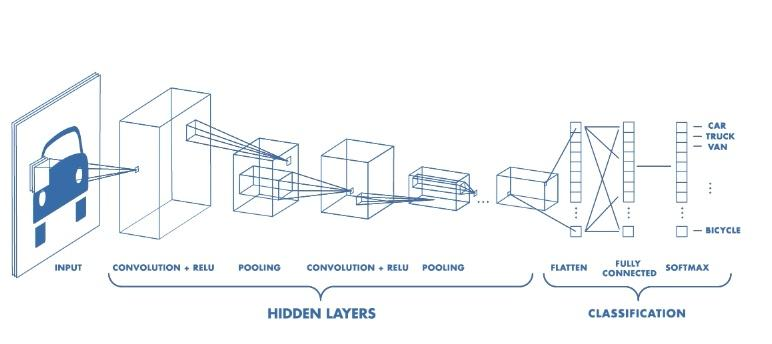
\includegraphics[scale=0.38]{卷积神经网络结构.jpg}
	\caption{卷积神经网络结构}
\end{figure}

一个卷积神经网络由若干卷积层(convolutional layer),池化层(pooling layer),全连接层(full connected layer)组成。
\begin{center}
	卷积神经网络的基本流程
\end{center}
\begin{itemize}
	\item[\textcircled{1}] 输入图像到输入层
	\item[\textcircled{2}] 第一个卷积层的输入图像通过卷积核加偏置进行卷积操作,得到特征图
	\item[\textcircled{3}] 在第一个卷积层之后,第一个池化层对特征图做下采样,得到更小的特征图
	\item[\textcircled{4}] 第二个卷积层,每个卷积核Fitler把前面下采样之后的特征图卷积在一起,得到新的特征图。
	\item[\textcircled{5}] 第二个池化层,对新的特征图进行下采样,得到更小的特征图
	\item[\textcircled{6}] 卷积神经网络的最后两层是全连接层。这些像素值连接成一个向量输入到传统的神经网络中,得到输出。
\end{itemize}

\subsection{卷积层(Convolution Layer)}

主要作用是对输入的特征图(或原始数据)进行特征提取(卷积操作),输出卷积后产生的特征图,而完成该功能的是卷积层中的卷积核(Filter)。卷积层是卷积神经网络的核心部分,卷积层的加入使得神经网络能够共享权重,就能进行局部感知,并开始层次化地对图像进行抽象理解。

\subsubsection{全连接层的问题}
前馈神经网络模型是使用全连接层堆叠的方式构造的,前一层的神经元与后一层的神经元是全部相连的。有两个问题:1.使用全连接层构造的前馈神经网络需要大量的参数,计算消耗巨大。2.输入数据的形状特征被忽略了,所有输入到全连接层的数据被拉平成一堆数据,相邻元素间的关联被破坏,无法利用与形状相关的信息
\subsubsection{卷积运算}
卷积(convolution)是泛函分析中一种重要的运算。在图像上,对图像用一个卷积核进行卷积运算,实际上是一个滤波的过程。卷积实际是提供一个权重模板,这个模板在图像上滑动,并将中心依次与图像中每一个像素对齐,然后对这个模板覆盖的所有像素进行加权,并将结果作为这个卷积核在图像上该点的响应。

如果输入的是一张图片,首先把输入图像分解成可以被卷积层处理的矩阵,把卷积核作用于输入的不同区域,然后产生对应的特征图。

在卷积网络中,每个稀疏过滤器通过共享权值都会覆盖整个可视域,这些共享权值的单元构成一个特征映射卷积核。

一方面,重复单元能够对特征进行识别,而不考虑它在可视域中的位置。另一方面,权值共享极大地减少需要学习地自由变量个数。

对三个色彩通道的输入图像进行卷积操作,我们可以将三通道的卷积过程看作是三个独立的单通道卷积过程,最后将三个独立的单通道卷积过程的结果进行相加,就得到了最后的输出结果。
\begin{figure}[htbp]
	\centering
	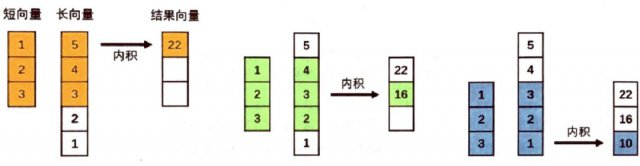
\includegraphics[scale=0.7]{一维卷积运算}
\end{figure}

随着短向量(卷积核)滑过输入信号,对应位置的元素相乘并计算出的总和作为相当窗口位置的输出,一般情况下卷积核的长度n远小于输入信号序列长度。

1.二维卷积

二维卷积在两个维度上以一定的间隔滑动二维滤波窗口,并在窗口内进行乘加运算,并将结果保存到输出对应的位置,从原矩阵的左上角开始计算卷积,当卷积核窗口滑过所有位置后二维卷积操作完成。

\begin{figure}[htbp]
	\centering
	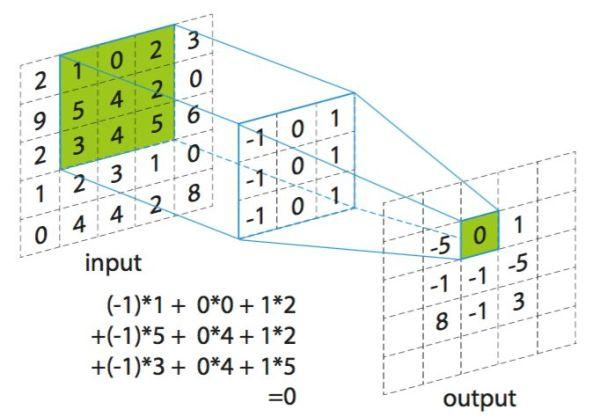
\includegraphics[scale=0.3]{卷积运算.jpg}
\end{figure}

在卷积神经网络中卷积核的参数对应全连接的权重,同时在卷积神经网络中也存在偏置。
\begin{figure}[htbp]
	\centering
	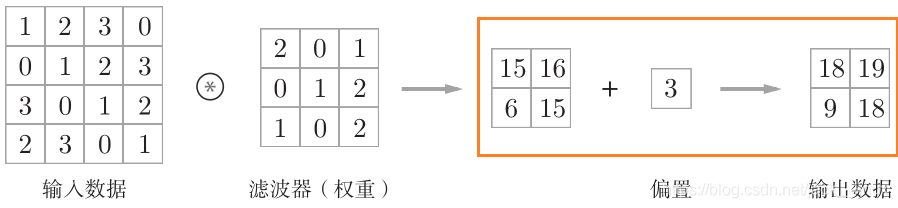
\includegraphics[scale=0.4]{卷积运算的偏置}
\end{figure}

2.填充(padding)

在对输入数据进行卷积操作之前,有时需要向输入数据周围补充一些固定的常数。主要目的是调整输入输出数据的大小,使得输入数据的形状与输出数据的形状保持一致,这样在卷积网络中才能一直堆叠卷积层,使得网络不断加深,否则输入数据不断变小,当输出数据的大小不如卷积核的大小时,就无法再进行卷积操作了。

\begin{figure}[htbp]
	\centering
	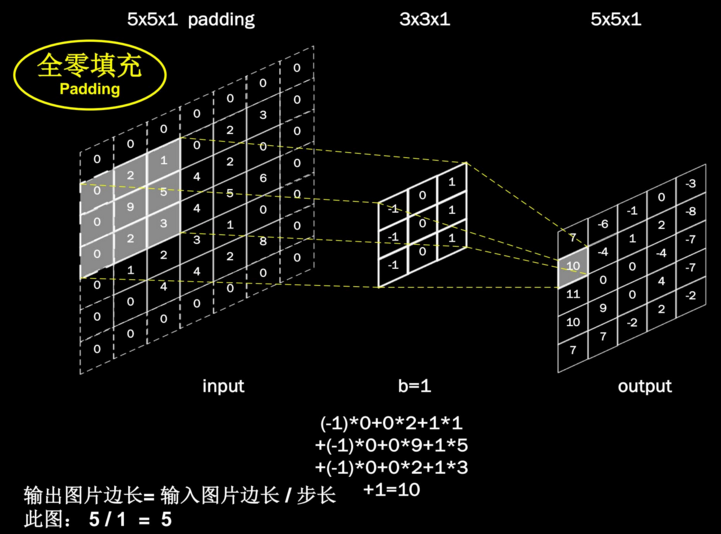
\includegraphics[scale=0.4]{零填充}
\end{figure}

有时候遇到每次移动步长较大,导致窗口的滑动出现不能刚好从头到尾的情况,故我们有两种边界像素填充方式:Valid和Same。Valid方式就是直接对输入图像进行卷积,不对输入图像进行任何前期处理和像素填充,缺点就是图像中的部分像素点无法被滑动窗口捕捉;Same方式是在输入图像的最外层加上指定数的值全为0的像素边界,这样就能让输入图像的所有的像素被滑动窗口捕捉。并且要注意步长应该适当。

如果补充的padding个数为偶数会在两侧补充相同个数个0,如果padding为奇数2n+1,会在左侧补n个0,右侧补n+1个0。
\begin{Python}{padding}
import tensorflow as tf
import numpy as np
tf.compat.v1.disable_eager_execution()
tf.compat.v1.reset_default_graph()
x = tf.compat.v1.placeholder(tf.float32, shape=(1, 50, 50, 1))
W1 = tf.compat.v1.get_variable('W1', shape=[3, 3, 1, 1], dtype=tf.float32, initializer=tf.ones_initializer())
W2 = tf.compat.v1.get_variable('W2', shape=[5, 5, 1, 1], dtype=tf.float32, initializer=tf.ones_initializer())
W3 = tf.compat.v1.get_variable('W3', shape=[7, 7, 1, 1], dtype=tf.float32, initializer=tf.ones_initializer())
W4 = tf.compat.v1.get_variable('W4', shape=[9, 9, 1, 1], dtype=tf.float32, initializer=tf.ones_initializer())
W5 = tf.compat.v1.get_variable('W5', shape=[11, 11, 1, 1], dtype=tf.float32, initializer=tf.ones_initializer())

conv1 = tf.nn.conv2d(x, W1, strides=[1, 1, 1, 1], padding='SAME')
conv2_same = tf.nn.conv2d(x, W2, strides=[1, 2, 2, 1], padding='SAME')
conv2_same_1 = tf.nn.conv2d(conv2_same, W2, strides=[1, 2, 2, 1], padding='SAME')
conv2_same_2 = tf.nn.conv2d(conv2_same_1, W2, strides=[1, 2, 2, 1], padding='SAME')
conv2_same_3 = tf.nn.conv2d(conv2_same_2, W2, strides=[1, 2, 2, 1], padding='SAME')

conv2_valid = tf.nn.conv2d(x, W2, strides=[1, 2, 2, 1], padding='VALID')
conv2_valid_1 = tf.nn.conv2d(conv2_valid, W2, strides=[1, 2, 2, 1], padding='VALID')
conv2_valid_2 = tf.nn.conv2d(conv2_valid_1, W2, strides=[1, 2, 2, 1], padding='VALID')

with tf.compat.v1.Session() as sess:
	feed_data = np.full((1, 50, 50, 1), 1)
	sess.run(tf.compat.v1.global_variables_initializer())
	[conv2_same, conv2_same_1, conv2_same_2, conv2_same_3] = sess.run([conv2_same, conv2_same_1, conv2_same_2, conv2_same_3], feed_dict={x: feed_data})
	[conv2_valid, conv2_valid_1, conv2_valid_2] = sess.run([conv2_valid, conv2_valid_1, conv2_valid_2], feed_dict={x: feed_data})
	
	conv2_same = conv2_same[0]
	conv2_same_map = []
	for i in range(len(conv2_same)):
	for j in range(len(conv2_same)):
	conv2_same_map.append(conv2_same[i][j][0])
	width = height = int(np.sqrt(len(conv2_same_map)))
	conv2_same = np.reshape(conv2_same_map, (width, height))
	print("padding = SAME")
	print("第一次卷积后特征图的尺寸:", len(conv2_same), "×", len(conv2_same))
	#	print(conv2_same)
	print("******************************************************")
	
	conv2_same_1 = conv2_same_1[0]
	conv2_same_1_map = []
	for i in range(len(conv2_same_1)):
	for j in range(len(conv2_same_1)):
	conv2_same_1_map.append(conv2_same_1[i][j][0])
	width = height = int(np.sqrt(len(conv2_same_1_map)))
	conv2_same_1 = np.reshape(conv2_same_1_map, (width, height))
	print("第二次卷积后特征图的尺寸:", len(conv2_same_1), "×", len(conv2_same_1))
	#	print(conv2_same_1)
	print("******************************************************")
	
	conv2_same_2 = conv2_same_2[0]
	conv2_same_2_map = []
	for i in range(len(conv2_same_2)):
	for j in range(len(conv2_same_2)):
	conv2_same_2_map.append(conv2_same_2[i][j][0])
	width = height = int(np.sqrt(len(conv2_same_2_map)))
	conv2_same_2 = np.reshape(conv2_same_2_map, (width, height))
	print("第三次卷积后特征图的尺寸:", len(conv2_same_2), "×", len(conv2_same_2))
	#	print(conv2_same_2)
	print("*****************************************************")
	
	conv2_same_3 = conv2_same_3[0]
	conv2_same_3_map = []
	for i in range(len(conv2_same_3)):
	for j in range(len(conv2_same_3)):
	conv2_same_3_map.append(conv2_same_3[i][j][0])
	width = height = int(np.sqrt(len(conv2_same_3_map)))
	conv2_same_3 = np.reshape(conv2_same_3_map, (width, height))
	print("第四次卷积后特征图的尺寸:", len(conv2_same_3), "×", len(conv2_same_3))
	#	print(conv2_same_3)
	print("***************************************************\n")
	
	conv2_valid = conv2_valid[0]
	conv2_valid_map = []
	for i in range(len(conv2_valid)):
	for j in range(len(conv2_valid)):
	conv2_valid_map.append(conv2_valid[i][j][0])
	width = height = int(np.sqrt(len(conv2_valid_map)))
	conv2_valid = np.reshape(conv2_valid_map, (width, height))
	print("padding=VALID")
	print("第一次卷积后特征图的尺寸:", len(conv2_valid), "×", len(conv2_valid))
	#	print(conv2_valid)
	print("******************************************************")
	
	conv2_valid_1 = conv2_valid_1[0]
	conv2_valid_1_map = []
	for i in range(len(conv2_valid_1)):
	for j in range(len(conv2_valid_1)):
	conv2_valid_1_map.append(conv2_valid_1[i][j][0])
	width = height = int(np.sqrt(len(conv2_valid_1_map)))
	conv2_valid_1 = np.reshape(conv2_valid_1_map, (width, height))
	print("第二次卷积后特征图的尺寸:", len(conv2_valid_1), "×", len(conv2_valid_1))
	#	print(conv2_valid_1)
	print("******************************************************")
	
	conv2_valid_2 = conv2_valid_2[0]
	conv2_valid_2_map = []
	for i in range(len(conv2_valid_2)):
	for j in range(len(conv2_valid_2)):
	conv2_valid_2_map.append(conv2_valid_2[i][j][0])
	width = height = int(np.sqrt(len(conv2_valid_2_map)))
	conv2_valid_2 = np.reshape(conv2_valid_2_map, (width, height))
	print("第三次卷积后特征图的尺寸:", len(conv2_valid_2), "×", len(conv2_valid_2))
	#	print(conv2_valid_2)
	print("******************************************************")


#OUTPUT:
#		padding = SAME
#		第一次卷积后特征图的尺寸: 25 × 25
#		***************************************************************
#		第二次卷积后特征图的尺寸: 13 × 13
#		***************************************************************
#		第三次卷积后特征图的尺寸: 7 × 7
#		***************************************************************
#		第四次卷积后特征图的尺寸: 4 × 4
#		***************************************************************
#		
#		padding=VALID
#		第一次卷积后特征图的尺寸: 23 × 23
#		***************************************************************
#		第二次卷积后特征图的尺寸: 10 × 10
#		***************************************************************
#		第三次卷积后特征图的尺寸: 3 × 3
#		***************************************************************
\end{Python}
试验中我们采用50x50的全为1的矩阵作为卷积输入,采用5x5的卷积核,步长为2。
$$ \text{输出长度}=\left\{ \begin{array}{cl}
	\displaystyle{\frac{\text{入长}}{\text{步长}}(\text{向上取整})}& : padding =SAME(\text{全0填充})\vspace{1ex}  \\
	
	\displaystyle{\frac{\text{入长}-\text{核长}+1}{\text{步长}}(\text{向上取整})}& : padding =VALID(\text{不全0填充})
\end{array} \right.$$
3.步长(stride)

步长(stride)是指卷积核窗口滑动的位置间隔。步长和填充都会改成卷积输出数据的大小,总结出以通用公式:用于计算输入图像经过一轮卷积操作后输出图像的宽度和高度的参数:
$$W_{output}=\frac{W_{input}-W_{filter}+2P}{S}+1$$
$$H_{output}=\frac{H_{input}-H_{filter}+2P}{S}+1$$

W和H分别表示图像的宽度(Weight)和高度(Height)的值;S表示卷积核的步长;P表示在图像边缘增加的边界像素层数,如果选择Same模式,则P(Padding)为图像增加的边界层数,如果选择的是Valid模式,P=0。input,output,filter分别表示输入图像,输出图像,卷积核的相关参数。

以下计算输出长度的计算公式中的增加的边界像素层:

1.padding = “VALID”:(不补0)P=0

2.padding = “SAME”:(补0)

卷积核的尺度为奇数:
$$P = (F-1)/2$$
Filter=1x1时,P=0;
Filter=3x3时,P=1;
Filter=5x5 时,P=2,以此类推。算出P回代上式得到输出。

\textcolor{red}{卷积核的尺寸为偶数:}
Filter=6x6时,P1=$((6-1)/2=2.5\approx 3)$向上取整,P2=$((6-1)/2=2.5\approx 2)$向下取整;当步长为大于1的数时,计算N的公式,一律向下取整,这样可以正确计算N的大小。

卷积神经网络中有几种常见的卷积形式:

(1)窄卷积(narrow convolition):步长s=1,填充p=0

(2)宽卷积(wide convolution):步长s=1,填充p=w-1

(3)等长卷积(equal-width convolution):步长s=1,填充p=(w-1)/2

实例:输入为$7\times7\times1$的图像数据,卷积核窗口为$3\times3\times1$,输入图像的最外层使用了一层边界像素填充(P=1),卷积核的步长stride为1,就可以得到$W_{output}=7$,$H_{output}=7$,P=1,S=1.然后根据公式就能够计算出最后输出特征图的宽度和高度都是7。

零填充填几层卷积层要自己计算的(计算是在滑动窗口滑动之前就计算好的)。例如:输入为$7\times7$的图像数据,卷积核窗口为$5\times3$,卷积核的步长stride为3,输入图像的最外层使用了一层边界像素填充(P=1),由上述的通用公式就可以得到$W_{output}=\frac{7}{3}$,$H_{output}=\frac{7}{3}$;输入图像的最外层使用了一层边界像素填充(P=2),由上述的通用公式就可以得到$W_{output}=3$,$H_{output}=3$。

4.转置卷积

在全连接层中,如果忽略激活函数,那么全连接层的前向计算和反向传播就是一种转置关系。在前向传播时,第l+1层的净输入为$z^{l+1} = \textbf{W}^{l+1}z^l$;在反向传播时,第l层的误差项为$\delta^l=(\textbf{W}^{l+1})^T\delta^{l+1}$。

卷积层可以看成全连接层的一种,其他连接的权重为0,可以将卷积操作也写成仿射变换的形式,假设卷积核$w=[w_1,w_2,w_3]^T$作用于一个4维的输入向量x上,输出2维的向量$z=[z_1,z_2]^T$。
$$z = w \bigotimes x= \begin{bmatrix}
	w_1 & w_2 &w_3  &0  \\
	0 & w_1 &w_2  & w_3
\end{bmatrix} \bullet \begin{bmatrix}
x_1 \\
x_2 \\
x_3 \\
x_4
\end{bmatrix} =\begin{bmatrix}
x_1w_1+x_2w_2+x_3w_3 \\x_2w_1+x_3w_2+x_4w_3 
\end{bmatrix}= Cx$$

仿射变换矩阵C由卷积核W中的元素构成,其他位置补0。若希望从低维的向量z向高维向量x的映射,可以通过仿射矩阵的转置来实现。
$$x = w^T \bigotimes z = \begin{bmatrix}
	w_1 & 0\\
	w_2  &w_1  \\
	w_3 & w_2 \\
	0  & w_3
\end{bmatrix} \bullet \begin{bmatrix}
	z_1 \\
	z_2 \\
\end{bmatrix} =\begin{bmatrix}
	w_1z_1 \\
	w_2z_1+w_1z_2\\
	w_3z_1+w_2z_2\\
	z_2w_3 
\end{bmatrix}= C^Tz$$
但是这里的转置矩阵并不是正定矩阵,只是一种转置上的形式,由这种形式上的转置将从低维向高维特征映射的卷积操作称为转置卷积(transposed convolution)或称反卷积(deconvolution)

在卷积操作中,可以通过增加卷积的步长s>1来对输入的特征进行降采样,反之可以通过减少转置卷积的步长s'=1/s来进行上采样。步长s<1的转置卷积称为微步卷积(fractionally-strided convolution)可以通过在输入特征之间插入0来间接地减少步长。
\begin{figure}[htbp]
	\centering
	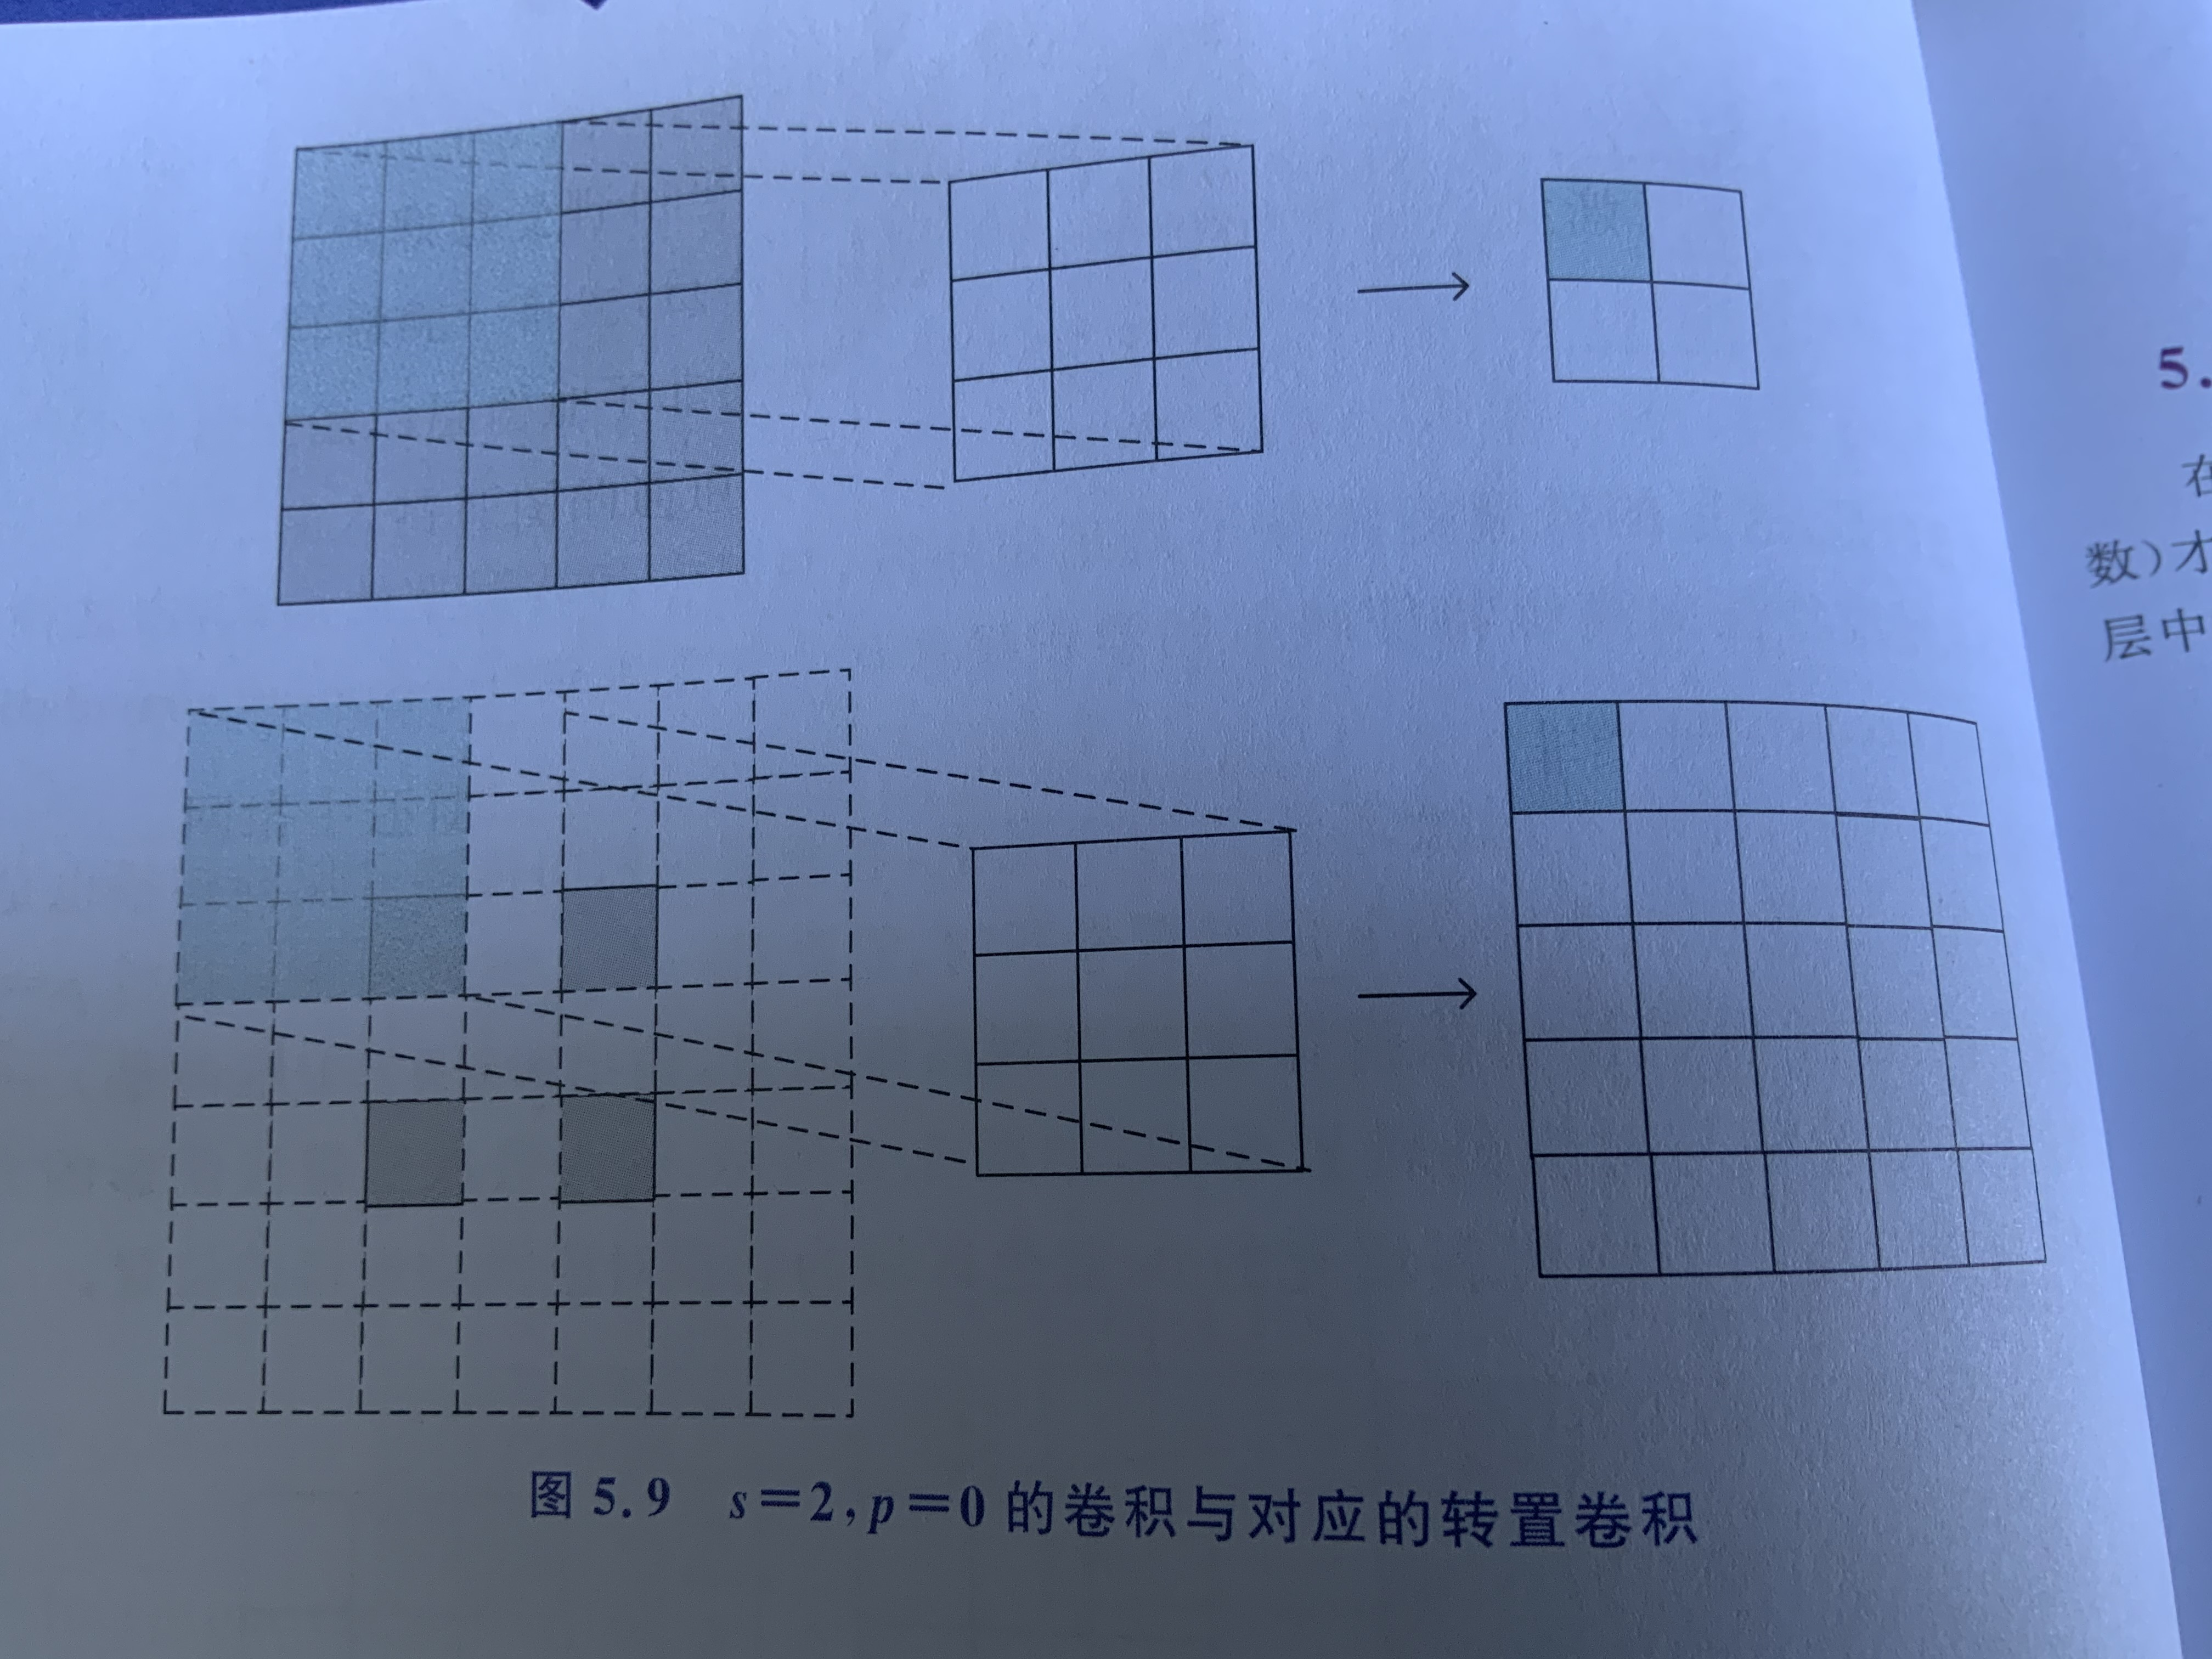
\includegraphics[scale=0.05]{转置卷积}
\end{figure}

如上图所示,先进行步长为2填充为0的降采样,得到$2\times 2$的输出。而转置卷积时的转置卷积步长为s'=1/s=0.5小于1,这时就要对n维向量z进行p=k-1的0填充操作,并且在输入特征的每两个向量之间插入$\frac{1}{s}-1$个0,通过步长为1的正常卷积操作来上采样到高维向量,其输出的大小为(n-1)s+k。

5.空洞卷积(atrous convolutions)

也称膨胀卷积(dilated convolution),是保留原始卷积参数数目的同时增加输出单元感受野的一种特殊卷积。空洞卷积在卷积核中填充0使得卷积核膨胀。

假设膨胀率为d,则需要在卷积核的每两个元素之间插入d个孔,原始卷积核大小为k,卷积核的有效大小为(k-1)d+k。
\begin{figure}
	\centering
	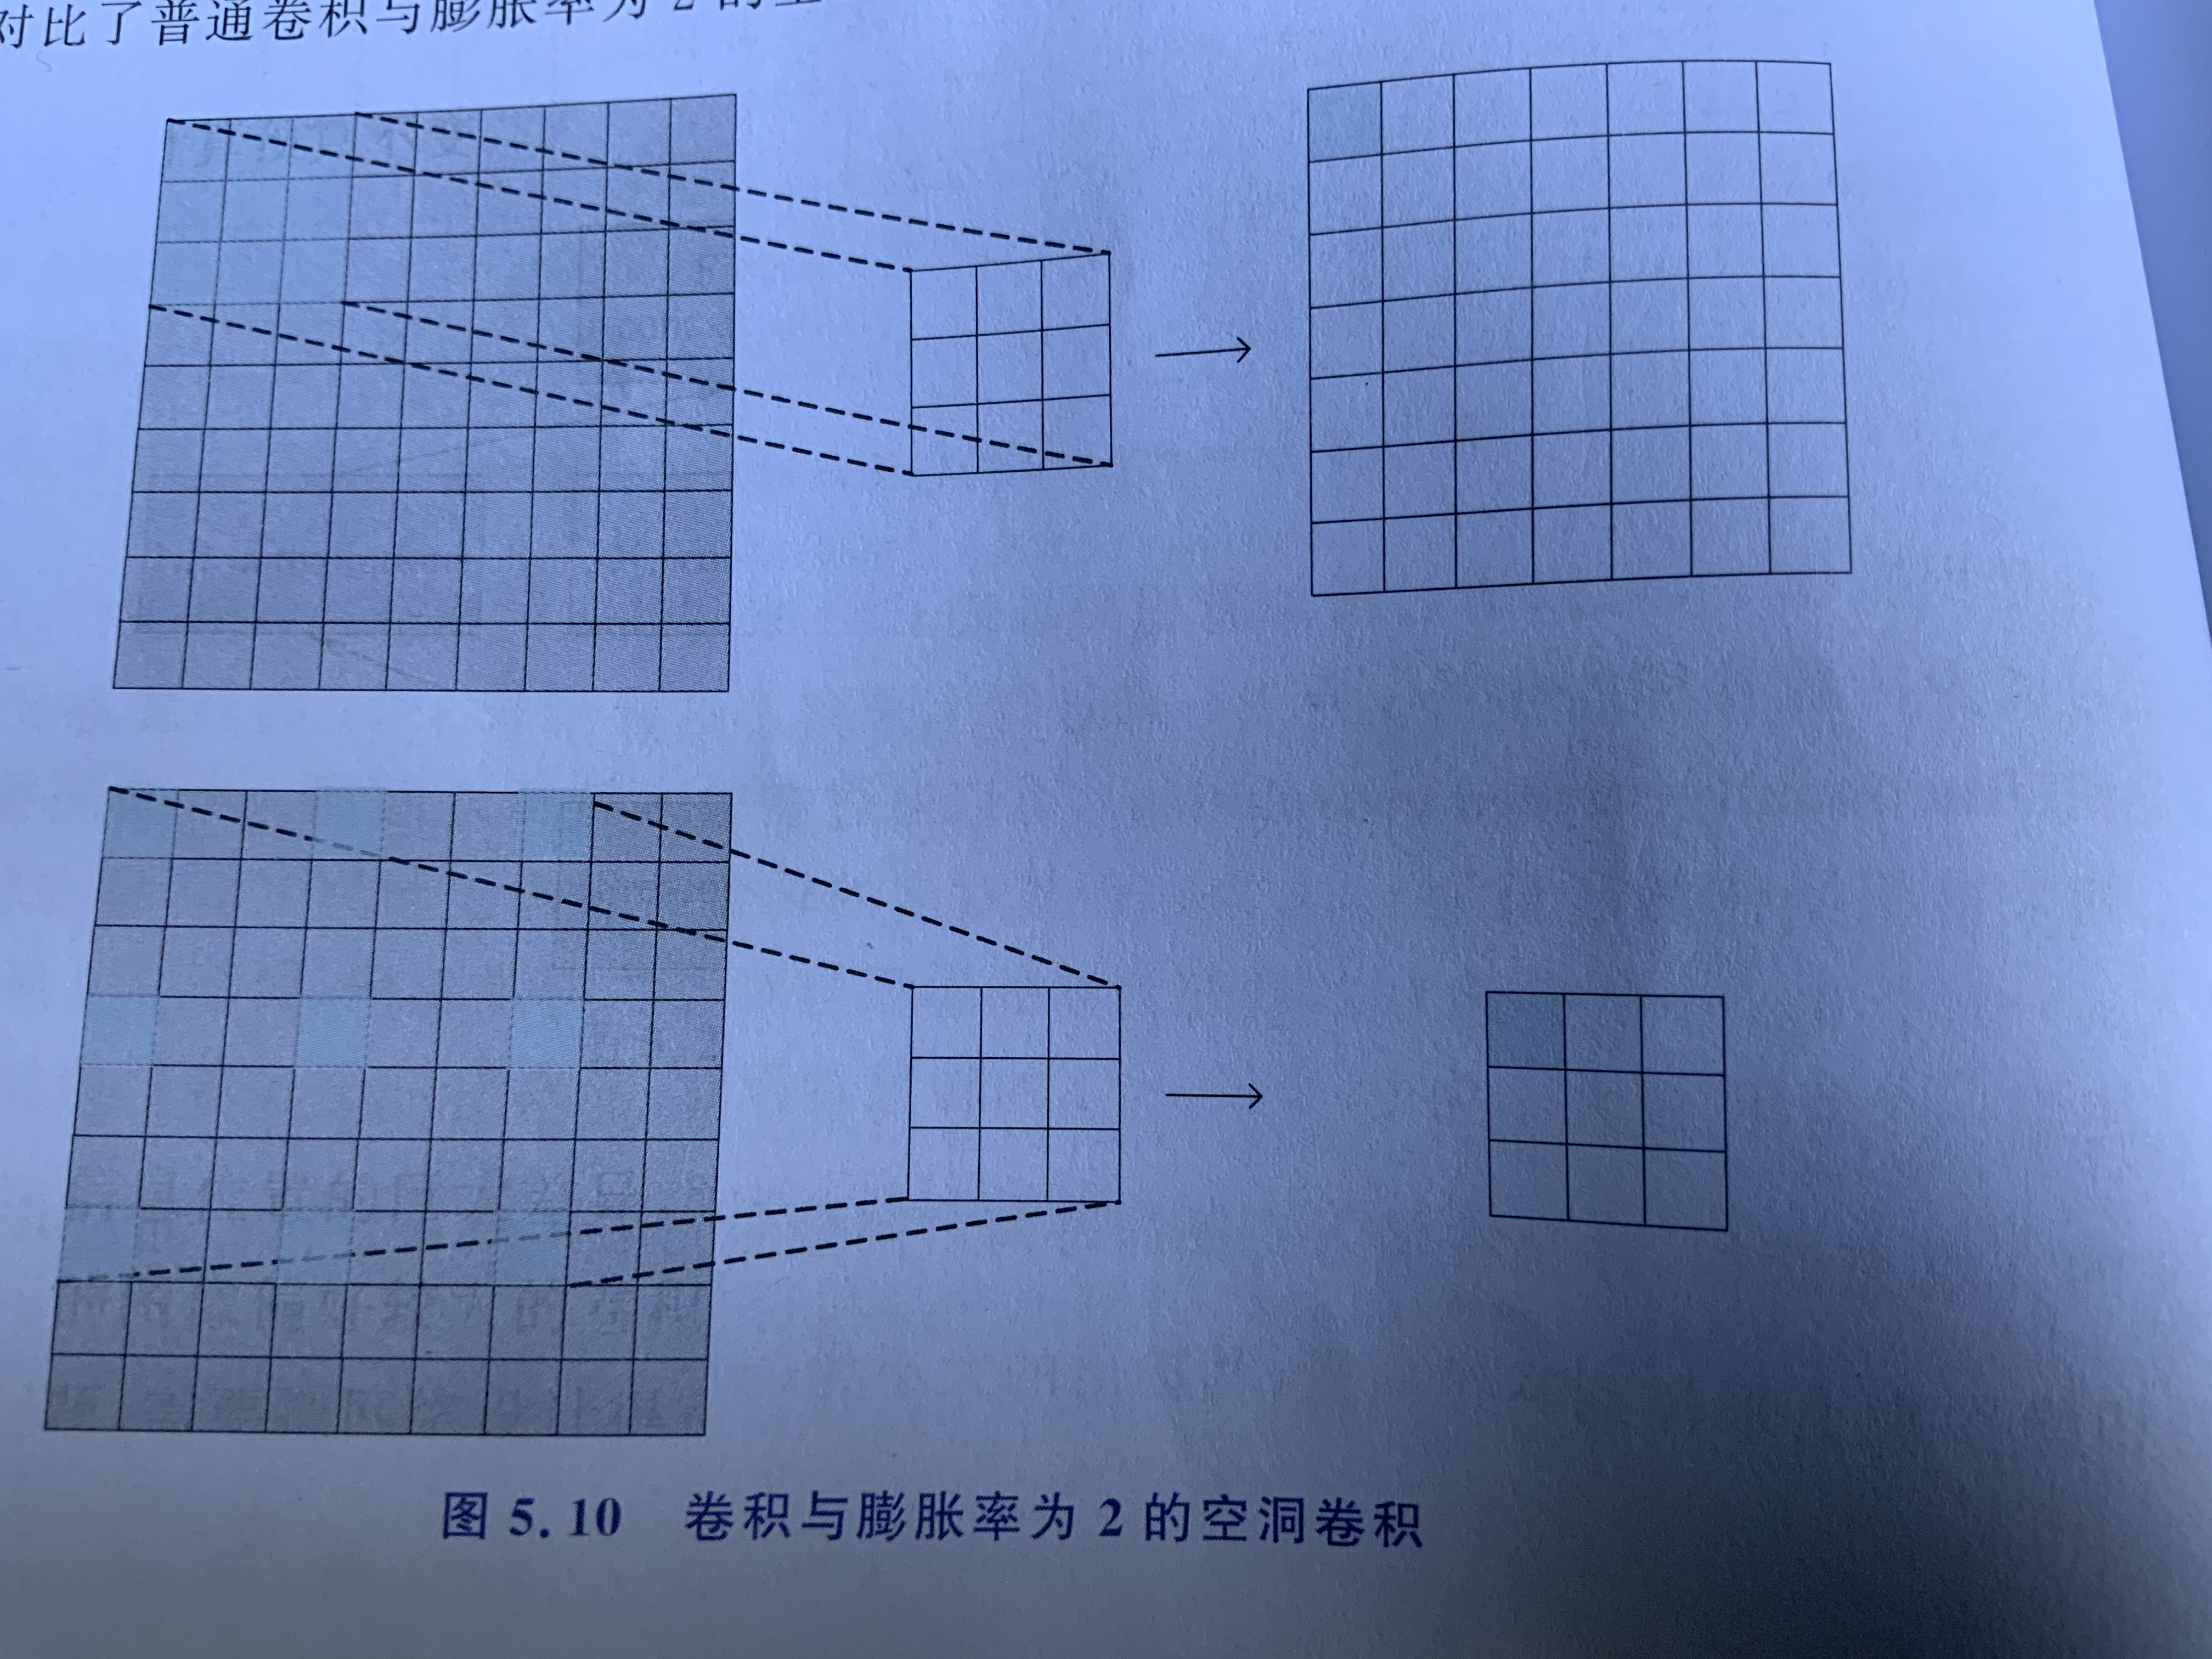
\includegraphics[scale=0.05]{空洞卷积}
\end{figure}

\subsubsection{卷积的导数}

反向传播算法,需要对全连接层中的各个参数求导数才能继续让误差反向流过全连接层。对卷积层,当误差反向传播时同样需要计算卷积层中参数的导数以保证误差反向传播的进行。

假设$Y=W\bigotimes X$,其中$x \in R^{H\times W},W\in R^{h\times w},Y\in R^{(H-h+1)\times (W-w+1)}$。
$$y_{i,j} = \sum_{u=1}^{m}\sum_{v=1}^{n}w_{u,v}x_{i+u-1,j+v-1}=\sum_{p=1}^{m}\sum_{q=1}^{n}x_{p,q}w_{p-i+1,q-j+1}$$
存在函数$f(Y)\in R$为标量函数,使得:
$$\frac{\partial f(Y)}{\partial w_{uv}}=\sum_{i=1}^{H-h+1}\sum_{j=1}^{W-w+1}\frac{\partial f(Y)}{\partial y_{ij}}\frac{\partial y_{ij}}{\partial w_{uv}}=\sum_{i=1}^{H-h+1}\sum_{j=1}^{W-w+1}\frac{\partial f(Y)}{\partial y_{ij}}\bullet x_{i+u-1,j+v-1}$$
$$\frac{\partial f(Y)}{\partial x_{pq}}=\sum_{i=1}^{H-h+1}\sum_{j=1}^{W-w+1}\frac{\partial f(Y)}{\partial y_{ij}}\frac{\partial y_{ij}}{\partial x_{pq}}=\sum_{i=1}^{H-h+1}\sum_{j=1}^{W-w+1}\frac{\partial f(Y)}{\partial y_{ij}}\bullet w_{p-i+1,q-j+1}$$

注意此时可能会出现边界溢出的情况,若p-i+1<1或者p-i+1>H或者q-j+1<1或者q-j+1>M,应对w和p=(H-h,W-w)的零填充,使$w_{p-i+1,q-j+1}=0$,这两者为反着遍历卷积核的,为了与之前的顺序与形式保持一致,可将卷积核作180度的翻转。即:
$$\frac{\partial f(Y)}{\partial x_{pq}}=rot180(w)\bigotimes \frac{\partial f(Y)}{\partial w_{uv}}$$

\subsubsection{卷积层操作}
一般情况下输入特征图(C,H,W)的通道数C与卷积核(KC,KH,KW)的通道数KC相等,无须在通道方向滑动。

\begin{figure}[htbp]
	\centering
	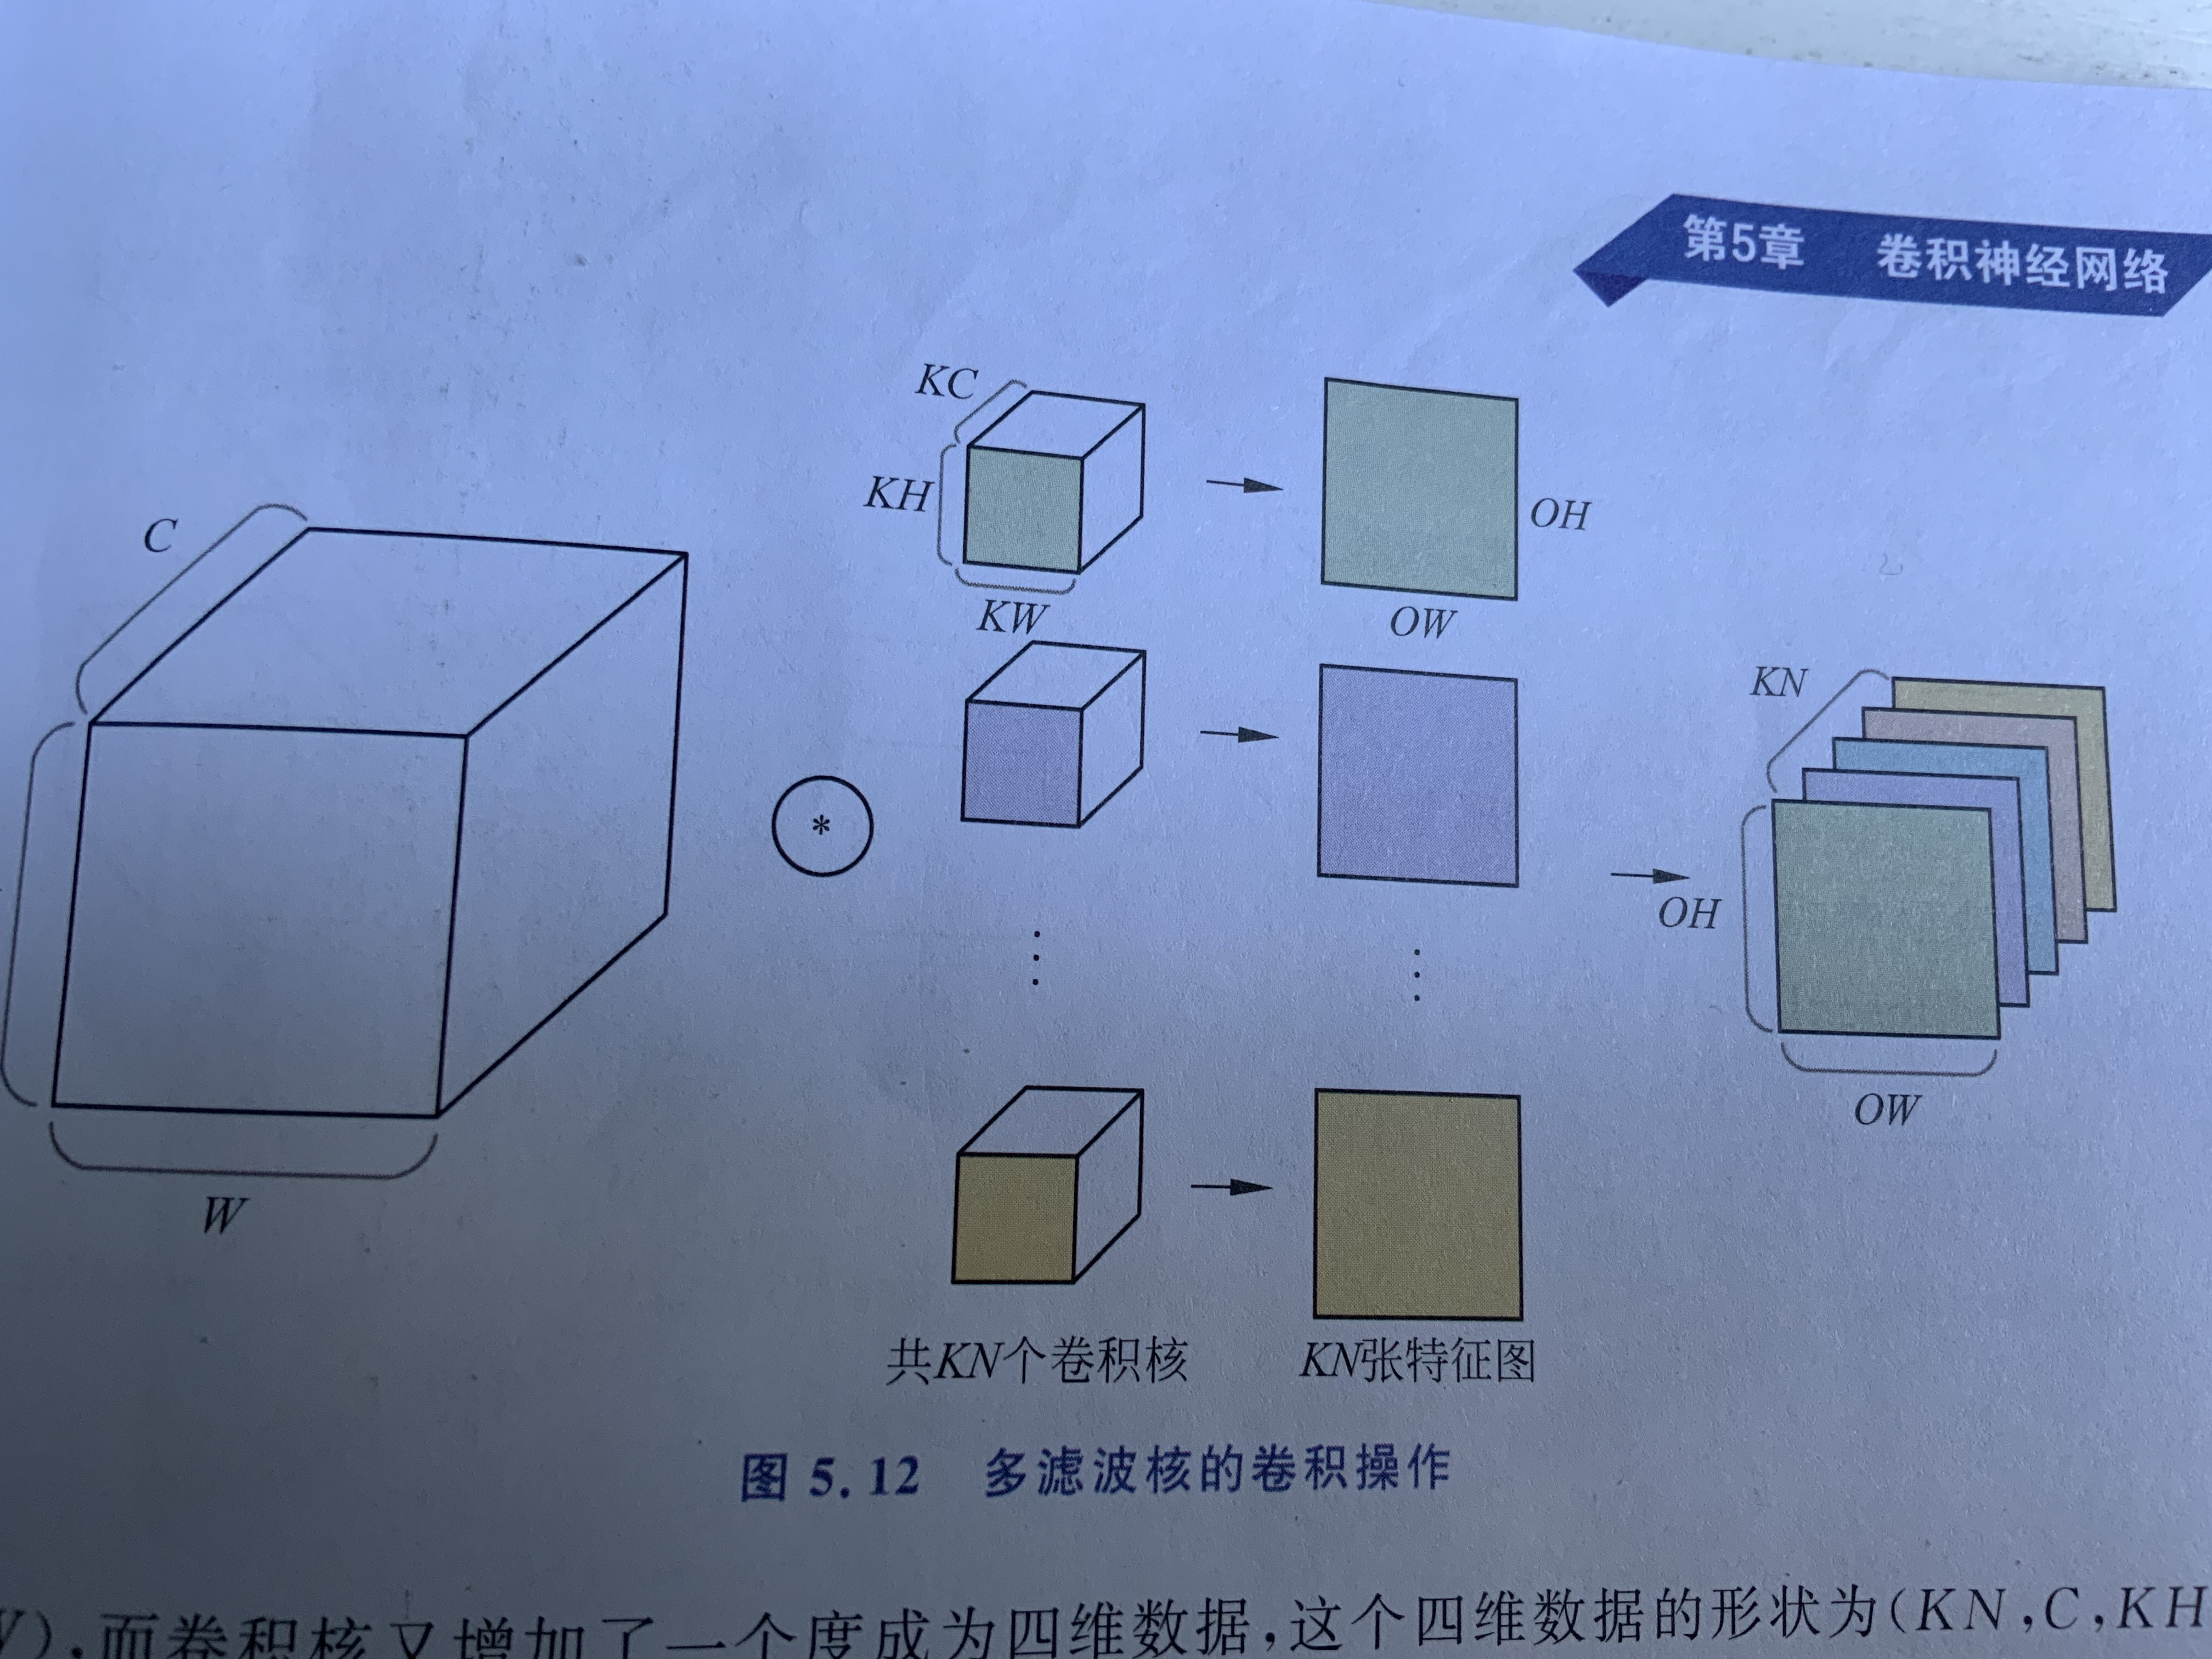
\includegraphics[scale=0.08]{多滤波核的卷积操作}
\end{figure}
图中使用了KN个不同的卷积核,共产生了KN张特征图,输出数据的形状为(KN,OH,OW),而卷积核又增加了一个维度成为四维数据,这个数据的形状为(KN,C,KH,KW)。

卷积核第一维的大小决定输出数据的通道数$C_{out}$,第二维的大小由输入数据的通道数$C_{in}$决定,卷积核中参数的数量为$C_{out}\times C_{in}\times KH\times KW$。

有时卷积层也可能存在偏置b,且每个通道中只有一个偏置,偏置第一维的长度等于输出特征图的通道数,其形状维(KN,1,1)

在训练神经网络时为了加快运算速度,通常会使用mini-batch,卷积神经网络能够一次对N数据进行批处理,此时输入/输出特征图按(Mini\_batch,Channel.Height,Width)的形式保存数据。

1.局部感知

卷积操作关注的是局部的像素,一个神经元只与局部区域中的像素相连,而全连接层中一个神经元的感受野覆盖了全部输入。局部连接方式保留了输入数据原有的空间联系,保留了数据中的一些模式,随着网络加深,每个神经元的感受野逐渐增大,对图像的提取也从局部到整体。保证了学习后的卷积核能够对局部的输入特征有最强的响应。

2.权重共享

权重共享是指卷积核在滑动过整个图像的时候,卷积核的参数不变。这样能够极大地减少参数。权重只是对于同一通道地神经元共享。偏重对所有神经元都是共享的。

\subsubsection{矩阵快速卷积}
卷积运算通过在输入特征图上滑动窗口,逐步长地进行窗口内元素的乘加运算,会消耗大量的资源和时间在数据寻址和内存数据读写上。可以将特征图和卷积核展开,形成两个二维矩阵,并以矩阵乘的方式进行。
\begin{figure}[htbp]
	\centering
	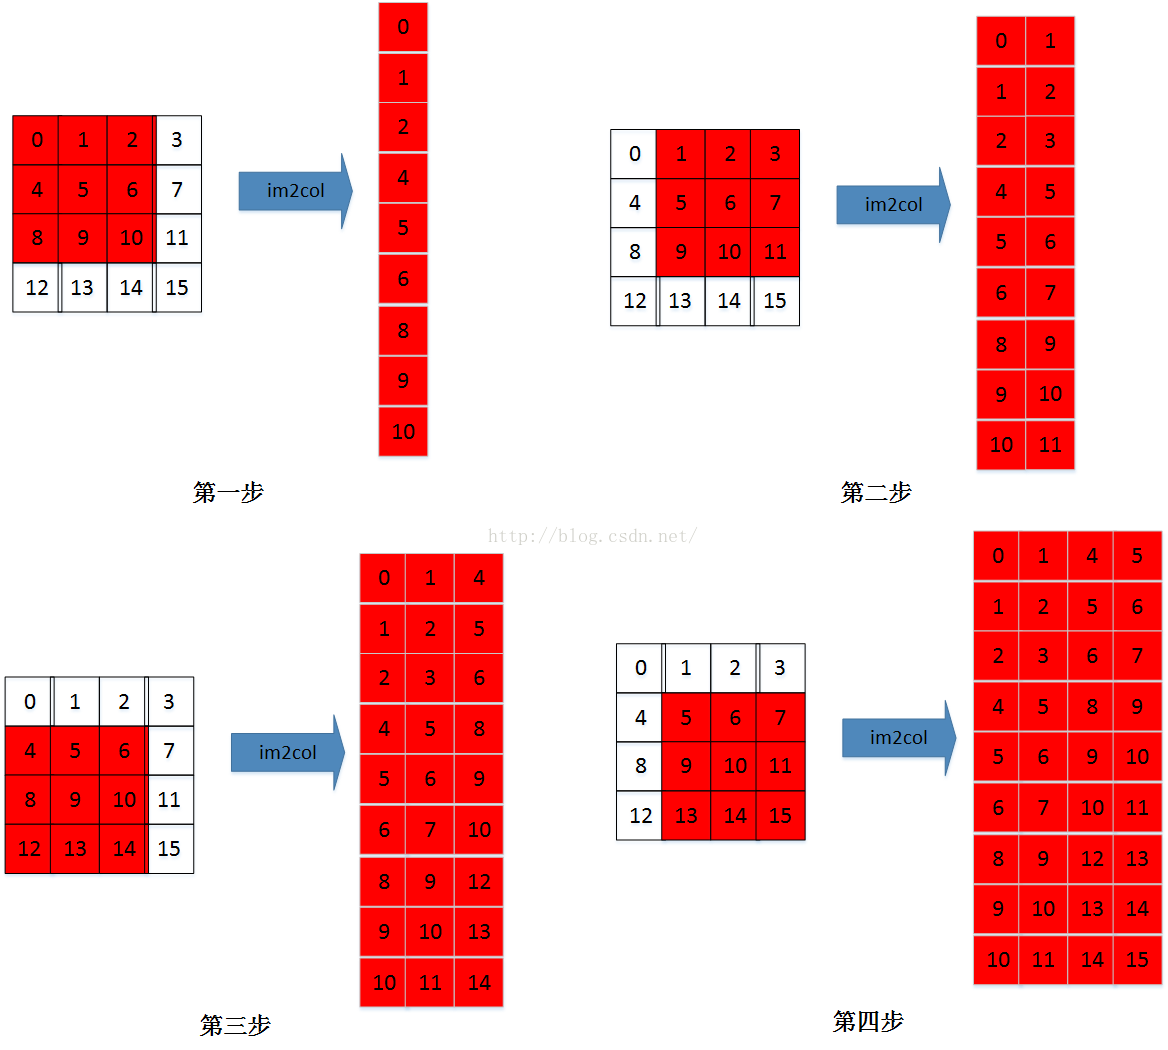
\includegraphics[scale=0.3]{im2col}
\end{figure}
\subsection{池化层}
池化层被看作是卷积神经网络中的一种提取输入数据的核心特征的方式,不仅实现了对原始数据的压缩,还大量减少了参与模型计算的参数,从某种意义上提升了计算效率。池化层的输入一般来源于上一个卷积层,主要是提供很强的鲁棒性并且减少参数的数量,防止过拟合现象的发生。

池化层最常用的方法包括最大池化和平均池化,主要是用来降低网络的复杂度。池化层处理的输入数据在一般情况下是经过卷积操作之后生成的特征图。

平均池化:如果取区域均值(Meaning-pooling),往往能保留整体数据的特征,能突出背景的信息。滑动窗口依旧是步长为2的$2\times2$的窗口,有时窗口尺寸为$3\times 3$。更大的窗口尺寸比较罕见,因为过大的滑窗会急剧减少特征的数量,造成过多的信息损失。

最大池化:如果取区域最大值(Max-pooling)能更好的保留纹理上的特征。滑动窗口依旧是步长为2的$2\times2$的窗口,滑动窗口的深度核特征图的深度保持一致。例如:由于是取一个小区域的最大值,此区域中其他值变化,或图像稍有移动,但pooling后的结果不变。

\begin{figure}[htbp]
	\centering
	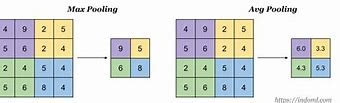
\includegraphics[scale=1]{4-4}
\end{figure}

通过池化层的计算输入的特征图经过一轮池化操作后输出的特征图的宽度和高度:
$$W_{output}=\frac{W_{input}-W_{filter}}{S}+1$$
$$H_{output}=\frac{H_{input}-H_{filter}}{S}+1$$

其中,W和H分别表示特征图的宽度和高度值,下标input,output和filter表示输入,输出的特征图和滑动窗口的相关参数,S表示胡山东窗口的步长,并且输入的特征图的深度和滑动窗口的深度保持一致。

例如:定义一个$16\times16\times6$的输入图像,池化层的滑动窗口为$2\times2\times6$,滑动窗口的步长stride=2,这样可以得到$W_{input}=16,H_{input}=16,W_{filter}=2,S=2$,计算可得输出特征图的宽度和高度都为8。池化层不仅能够最大限度地提取输入地特征图的核心特征,还能够对输入地特征图进行压缩。
\subsection{归一化层}
批归一化(Batch Normalization,BN)在深度网络各层之间进行数据批量归一化的算法,以解决深度神经网络内部方差偏移(Internal Covariate Shift)问题,使用网络训练过程中各层梯度的变化趋于稳定,并使网络在训练时能够更快地收敛。BN算法一般作为独立的层灵活地嵌在深度神经网络地各层之间,在与卷积层结合时,BN层一般位于卷积层和激活函数之间。

所谓的内部协方差偏移是由于深度神经网络中每层的输入总在不断变化,导致每层的参数需要不断更新以适应输入的新分布。批归一化就是将每层的数据强制拉回均值为0,方差为1的分布,使得各层的分布一致,训练过程也随之平衡。

BN能够减少训练时每层梯度的变化幅度,使梯度稳定在比较合适变化范围内,减少了梯度对参数的尺度与初始值的依赖,降低了调参的难度。可使网络训练时使用较大的学习率,加快网络的收敛速度。原因:$BN(Wu) \equiv BN((aW)u)$,故有:
$$\frac{\partial BN((aW)u)}{\partial u}=\frac{\partial Wu}{\partial u}$$
$$\frac{\partial BN((aW)u)}{\partial aW}=\frac{1}{a}\frac{\partial Wu}{\partial W}$$

BN表现出来的正则作用,也可以在训练时适当减少L2正则的权重。


输入:每个Mini-Batch中输入x的值$B={x_{1...m}}$,需要学习的参数$\gamma$,$\beta$

输出:BN结果{$y_i = BN_{\gamma \beta(x_i)}$}

BN具体算法过程:

1.对数据进行批归一化:
$$\mu_B\gets  \frac{1}{m}\sum_{i=1}^mx_i$$
$$\sigma_B^2\gets \frac{1}{m}\sum_{i=1}^m(x_i-\mu_B)^2$$
$$\hat{x}_i\gets\frac{x_i-\mu_B}{\sqrt{\sigma_b^2+\xi}}$$
此时一些激活函数的线性区减少了非线性,导致网络表达能力下降,增加了两个调节参数(scale)和(shift),这两个参数是通过学习得到。用来对归一化的数据进行反变换,增加了网络表达能力。

2.对批归一化后的数据进行一定的缩放和平移
$$y_i = \gamma\hat{x}_i+\beta \equiv BN_{\gamma \beta(x_i)}$$

BN在训练时可根据Mini-Batch里的数据统计均值和方差,推断时用的是全体训练样本中获得的统计量来进行操作。全局的均值和方差可以通过个Mini-Batch里的均值和方差来估计。
$$E[x] \gets E_B[\mu_B]$$
$$Var[x] \gets \frac{m}{m-1}E_B[\sigma_B^2]$$

所存在的问题:(1)受限于Batch Size的大小,当Batch Size太小时作用不明显。(2)不利于像素级图片生成任务。(3)对RNN等动态网络作用不大。(4)训练时和预测时统计量不一致。

优化算法:层归一化(Layer Normalization),实例归一化(Instance Normalization)和组归一化(Group Normalization)
\begin{figure}[htbp]
	\centering
	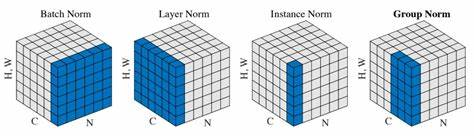
\includegraphics[scale=0.6]{归一化方法}
\end{figure}

层归一化:通过在单个训练样本中计算一层中所有神经元的响应的平均值和方差,然后对这些响应进行归一化操作。这使层归一化在训练和测试时执行完全一样的计算,更适用于循环神经网络等动态结构,在稳定循环网络中的隐状态方面非常有效。

实例归一化:进一步缩小了归一化统计量的计算范围,在CNN中对一层特征的某一通道计算平均值与方差,然后对这些响应进行归一化操作,重复操作直到此层所有通道完成归一化。

组归一化:在CNN中对一层特征图在通道维度进行分组,计算组内所有特征的均值与方差,然后对此组特征进行归一化操作,重复直到所有组完成归一化操作。
\subsection{全连接层}
全连接层能将输入图像在经过卷积和池化操作后提取的特征进行压缩,并且根据压缩的特征完成模型的分类功能。
\begin{figure}[htbp]
	\centering
	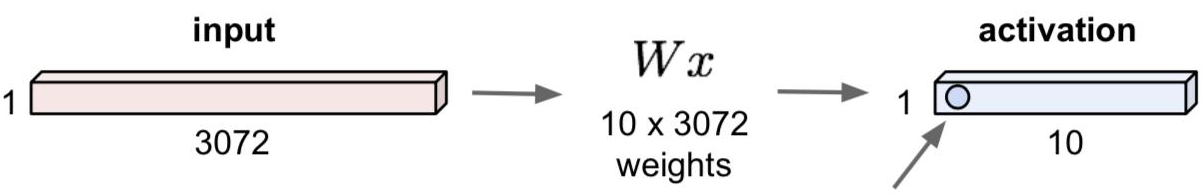
\includegraphics[scale=0.3]{4-6}
\end{figure}

输入的是我们通过卷积层和池化层提取的输入图像的核心特征,与全连接层中定义的权重参数相乘,最后被压缩成仅有的10个输出参数,在将10个参数输入到Softmax激活函数中进一步处理,激活函数的输出结果就是模型预测的输入图像对应各个类型的可能性值。

全连接会把卷积输出的二维特征图转化成一维的一个向量,全连接层的每个结点都与上一层的所有结点相连,用于把前边提取到的特征综合起来。全连接层就是高度提纯的特征,方便最后的分类器或者回归使用。
\subsection{参数学习}
卷积网络的参数学习可以通过误差反向传播算法来更新网络的参数。需要分别计算卷积层和池化层的误差项,得到误差项后进一步计算参数的梯度,卷积层中参数为卷积核以及偏置,池化层中没有参数,因此只需要更新卷积层中的参数。

(1)已知池化层的误差项$\delta^{l+1}$,求上一层误差项$\delta^l$

在前向传播算法中,一般会用最大函数和平均函数对输入进行池化操作,池化时滑窗的位置已知,在反向传播时,需要先把$\delta^{l+1}$的所有特征图大小还原成池化之前的大小,然后分配误差。
\begin{figure}[htbp]
	\centering
	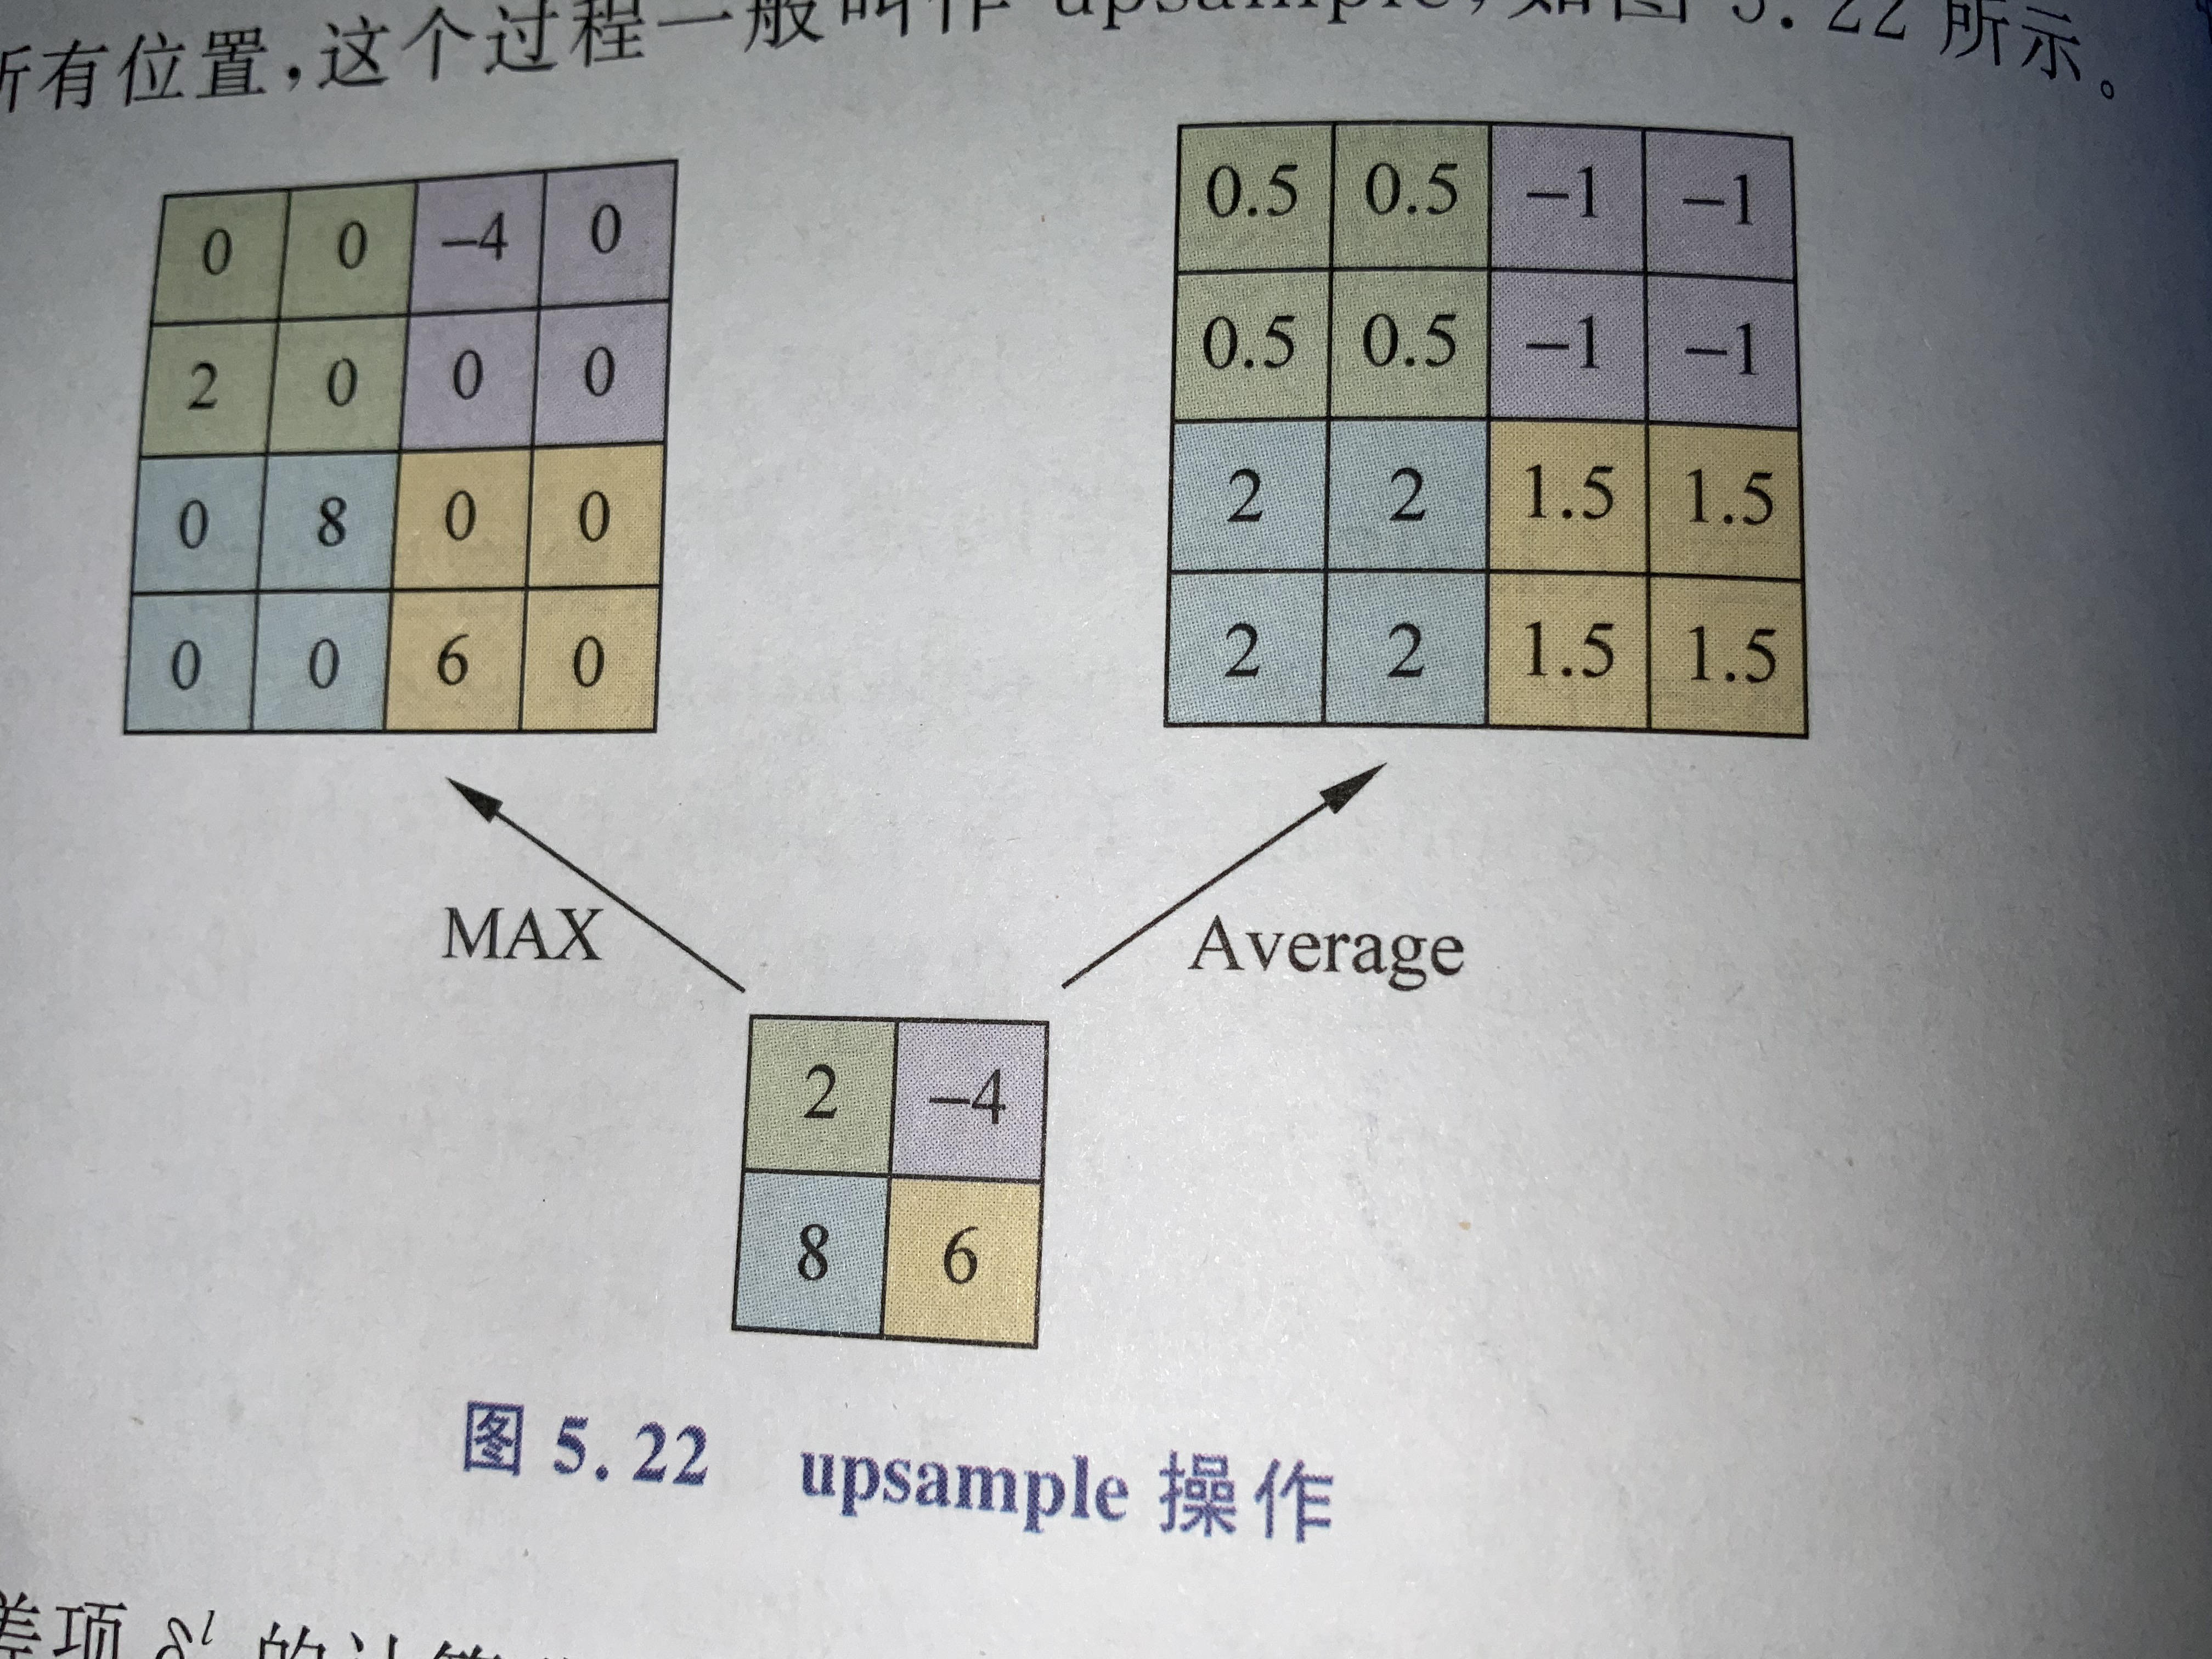
\includegraphics[scale=0.05]{upsample操作}
\end{figure}

若池化函数使用的是最大值函数MAX,则把$\delta^{l+1}$中特征图的各个值放在池化前最大值的位置。

若池化函数使用的是平均函数Average,则$\delta^{l+1}$中的特征图的各值平均分配到所有位置。

误差项$\delta^l$的计算公式:
$$\delta^{(l)}=\frac{\partial L(W,b)}{\partial Z^{(l)}}=upsample(\delta^{(l+1)})\odot f'(Z^{(l)})$$

池化层一般不再使用激活函数,或者认为$f(z)=z$,所以误差项$\delta^l$也直接写成:
$$\delta^{(l)}=upsample(\delta^{(l+1)})$$

(2)已知卷积层的误差项$\delta^{l+1}$,求上一层误差项$\delta^l$

设卷积神经网络中第l层的输入特征图为$X^{l-1}\in R^{C\times H\times W}$(一般输入从0开始编号),通过卷积操作后得到的净输入$Z^l\in R^{KN\times OH\times OW}$,第l层净输入中第c通道的特征图为:$$Z^{(l.c)}=W^{(l,c)}\otimes X^{l-1} + b^{(l,c)}$$
其中$W^{(l,t)}$第l层中的第c个卷积核权重,$b^{(l)}$为偏置。卷积神经网络中第l层的输出特征图(即第l+1层的输出特征图)为
$$X^{(l)}=f(z^{(l)})$$
其中f为激活函数。

卷积层中每个卷积核的运算都是一样的,则第l层中c通道的误差项$\delta^{(l,c)}$为
$$\delta^{(l,c)}=\frac{\partial L(W,b)}{\partial Z^{(l,c)}}=rot180(W^{(l+1,c)})\otimes \delta^{(l+1)}\odot f'(Z^{(l,c)})$$

卷积层中前向传播时卷积与误差反向传播时的卷积互为转置卷积。全连接层中前向传播时权重矩阵与误差分享传播时的矩阵互为转置矩阵。

由卷积层的误差项$\delta^{l,c}$,可以求出卷积层中权重$W^{(l,c)}$和偏置$c^{(l,c)}$的梯度:
\begin{equation*}
	\begin{aligned}
		\frac{\partial L(W,b)}{\partial W^{(l,c)}} &=\frac{\partial L(W,b)}{\partial Z^{(l,c)}}\otimes X^{(l-1)} \\
		&=\delta^{(l,c)}\otimes X^{(l-1)}
	\end{aligned}
\end{equation*}
$$\frac{\partial L(W,b)}{\partial b^{(l,c)}}=\sum_{i,j}\delta_{i,j}^{(l,c)}$$

\subsection{经典的卷积神经网络}

\subsubsection{ImageNet大规模视觉识别挑战赛}
ImageNet中含有超过1500万个由人工注释的图片网址,即带标签的图片,标签说明了图片中的内容,超过2.2万个类别。其中,至少有100万张里面提供了边框(Bounding Box)。2010年——2017年。

2012年:

AlexNet是2012年ImageNet竞赛冠军获得者Hinton和他的学生Alex Krizhevsky设计的。也是在那年之后,更多的更深的神经网络被提出,比如优秀的VGG,GoogLeNet。AlexNet中包含了几个比较新的技术点,也首次在CNN中成功应用了ReLU、Dropout和LRN等Trick。使用ReLU代替传统的Tanh或Logistic处理非线性的部分。在每个全连接层后面使用一个Dropout层,减少过拟合。

2013年:

OverFeat:OverFeat是早期经典的one-stage Object Detection的方法,基于AlexNet,实现了识别、定位、检测共用同一个网络框架;获得了2013年ILSVRC定位比赛的冠军。

OverFeat方法的主要创新点是 multiscale 、sliding window、offset pooling,以及基于AlexNet的识别、定位和检测方法的融合。

2014年:

GoogLeNet 冠军:从Inception v1到v4。引入稀疏特性和将全连接层转换成稀疏连接。在inception结构中,大量采用了1x1的矩阵,主要是两点作用:1)对数据进行降维;2)引入更多的非线性,提高泛化能力,因为卷积后要经过ReLU激活函数。

VGG(亚军):VGG模型在多个迁移学习任务中的表现要优于googLeNet。而且,从图像中提取CNN特征,VGG模型是首选算法。它的缺点在于,参数量有140M之多,需要更大的存储空间。

VGG的特点:
小卷积核。作者将卷积核全部替换为3x3(极少用了1x1);
小池化核。相比AlexNet的3x3的池化核,VGG全部为2x2的池化核;
层数更深特征图更宽。基于前两点外,由于卷积核专注于扩大通道数、池化专注于缩小宽和高,使得模型架构上更深更宽的同时,计算量的增加放缓;
全连接转卷积。网络测试阶段将训练阶段的三个全连接替换为三个卷积,测试重用训练时的参数,使得测试得到的全卷积网络因为没有全连接的限制,因而可以接收任意宽或高为的输入。

2015年:

ResNet:
残差网络的特点是容易优化,并且能够通过增加相当的深度来提高准确率。其内部的残差块使用了跳跃连接,缓解了在深度神经网络中增加深度带来的梯度消失问题 。

生成了ResNet-50,ResNet-101,ResNet-152. 随着深度增加,因为解决了退化问题,性能不断提升。作者最后在Cifar-10上尝试了1202层的网络,结果在训练误差上与一个较浅的110层的相近,但是测试误差要比110层大1.5\%。但是采用了太深的网络,发生了过拟合。

2016年:

Trimps-Soushen冠军

ResNeXt(亚军):
ResNeXt是ResNet[2]和Inception[3]的结合体,不同于Inception v4[4]的是,ResNext不需要人工设计复杂的Inception结构细节,而是每一个分支都采用相同的拓扑结构。ResNeXt的本质是分组卷积(Group Convolution)[5],通过变量基数(Cardinality)来控制组的数量。组卷机是普通卷积和深度可分离卷积的一个折中方案,即每个分支产生的Feature Map的通道数为 [公式]

2017年:

SENet是ImageNet 2017(ImageNet收官赛)的冠军模型,和ResNet的出现类似,都在很大程度上减小了之前模型的错误率),并且复杂度低,新增参数和计算量小。下面就来具体介绍一些SENet的神奇之处。

SENet的全称是Squeeze-and-Excitation Networks,中文可以翻译为压缩和激励网络。主要由两部分组成:

Squeeze部分。即为压缩部分,原始feature map的维度为HWC,其中H是高度(Height),W是宽度(width),C是通道数(channel)。Squeeze做的事情是把HWC压缩为11C,相当于把HW压缩成一维了,实际中一般是用global average pooling实现的。HW压缩成一维后,相当于这一维参数获得了之前H*W全局的视野,感受区域更广。

Excitation部分。得到Squeeze的11C的表示后,加入一个FC全连接层(Fully Connected),对每个通道的重要性进行预测,得到不同channel的重要性大小后再作用(激励)到之前的feature map的对应channel上,再进行后续操作。
\subsubsection{LeNet-5神经网络结构}
LeNet-5是一种典型的用来识别数字的卷积网络。LeNet-5共有7层,不包括输入,每层都包含可训练参数。
\begin{figure}[htbp]
	\centering
	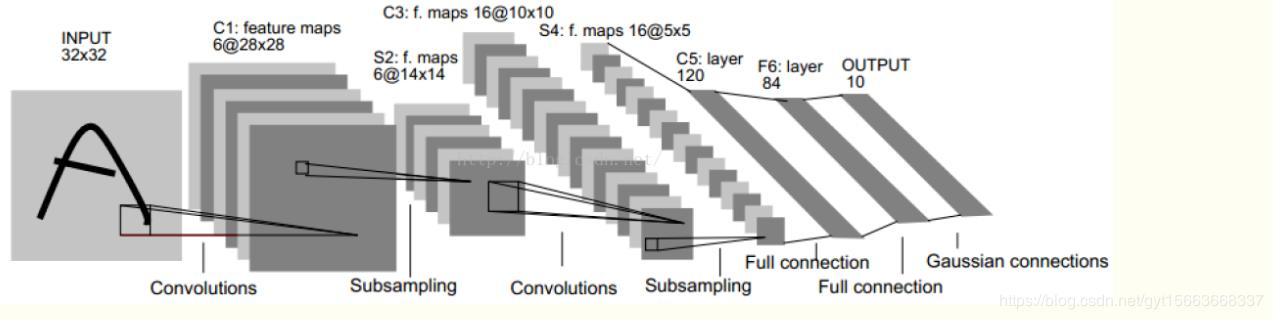
\includegraphics[scale=0.3]{LeNet-5神经网络结构.jpg}
\end{figure}

1.INPUT层:为输入层,默认输入数据必须是维度为$32\times32\times1$的图像,即输入的高度和宽度均为32的单通道图像

2.C1层:第一个卷积层,使用的卷积核滑动窗口为过$5\times5\times1$,步长为1,不使用Padding,如果输入数据的高度和宽度为32,则得到最后输出的特征图的高度和宽度为28,这个卷积层输出深度为6的特征图,故需要进行6次同样的卷积操作,最后得到输出的特征图的维度为$28\times28\times6$

3.S2层:下采样层,目的是缩减输入的特征图的大小,这里我们使用最大池化层来进行下采样。选择最大池化层的滑动窗口为$2\times2\times6$,步长为2。输入的特征图的高度和宽度均为28,可以得到最后输出的特征图的高度和宽度均为14,本层输出的特征图为$14\times14\times6$

4.C3层:第二个卷积层,因为卷积核滑动窗口的深度必须要与输入特征图的深度一致,输入的特征图维度为$14\times14\times6$故使用的卷积核滑动窗口为$5\times5\times6$,步长为1,不使用Padding,根据公式得到最后输出的特征图的高度和宽度为10,这个卷积层输出深度为16的特征图,故需要进行16次同样的卷积操作,最后得到输出的特征图的维度为$10\times10\times16$

5.S4层:下采样层,使用最大池化层来进行下采样,输入特征图的维度为$10\times10\times16$,最大池化层滑动窗口选择$2\times2\times16$,步长为2。得到最后输出的特征图的高度和宽度为5,特征图的维度为$5\times5\times16$

6.C5层:第三个卷积层,是之前的下采样层和之后的全连接层的一个中间层。使用的卷积核滑动窗口为$5\times5\times16$,步长为1,不适用Padding,得到最后输出的特征图的高度和宽度为1,这个卷积层输出深度为120的特征图,故需要进行120次同样的卷积操作,最后得到输出的特征图的维度为$1\times1\times120$

7.F6层:第一个全连接层,输入数据的维度为$1\times1\times120$的特征图,要求最后输出深度为84的特征图,故要进行压缩处理,就需要让输入的特征图乘上一个维度为$120\times84$的权重参数,最后维度为$1\times84$的矩阵为全连接层最后输出的特征图

8.OUTPUT层:解决的分类问题,输出的结果是输入图像对应10个类别的可能性值。先将F6层输入的维度为$1\times84$的数据压缩成维度为$1\times10$的数据,依靠一个$84\times10$的矩阵来完成。最终得到10个数据全部输入Softmax激活函数中,得到的就是模型预测的输入图像所对应10个类别的可能性值。
\subsubsection{AlexNet模型}
这个卷积神经网络模型的网络架构。
\begin{figure}[htbp]
	\centering
	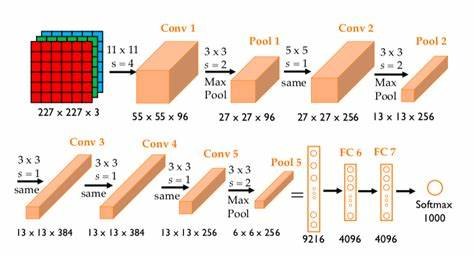
\includegraphics[scale=0.5]{AlexNet}
\end{figure}

(1)INPUT层:默认输入数据必须是维度为$224\times224\times3$的图像,即输入图像的高度和宽度均为224,色彩通道为R,G,B三个通道。

(2)Conv1层:第一个卷积层,使用的卷积核滑动窗口为$11\times11\times3$,步长为4,Padding为2,可得最后输出的特征图的高度核宽度均为55,这个卷积层输出深度为96的特征图,故需要进行96次同样的卷积操作,最后得到输出的特征图的维度为$55\times55\times96$

(3)MaxPool1层:第一个最大池化层。滑动窗口为$3\times3\times96$,步长为2,,可得最后输出的特征图的高度和宽度均为27,最后得到输出的特征图的维度为$27\times27\times96$

(4)Conv2层:第二个卷积层,使用的卷积核滑动窗口为$5\times5\times96$,步长为1,Padding为2,可得最后输出的特征图的高度核宽度均为27,这个卷积层输出深度为256的特征图,故需要进行256次同样的卷积操作,最后得到输出的特征图的维度为$27\times27\times256$

(5)MaxPool2层:第二个最大池化层。滑动窗口为$3\times3\times256$,步长为2,,可得最后输出的特征图的高度和宽度均为13,最后得到输出的特征图的维度为$13\times13\times256$

(6)Conv3层:第三个卷积层,使用的卷积核滑动窗口为$3\times3\times256$,步长为1,Padding为1,可得最后输出的特征图的高度核宽度均为13,这个卷积层输出深度为384的特征图,故需要进行384次同样的卷积操作,最后得到输出的特征图的维度为$13\times13\times384$

(7)Conv4层:第四个卷积层,使用的卷积核滑动窗口为$3\times3\times384$,步长为1,Padding为1,可得最后输出的特征图的高度核宽度均为13,这个卷积层输出深度为384的特征图,故需要进行384次同样的卷积操作,最后得到输出的特征图的维度为$13\times13\times384$

(8)Conv5层:第五个卷积层,使用的卷积核滑动窗口为$3\times3\times384$,步长为1,Padding为1,可得最后输出的特征图的高度核宽度均为13,这个卷积层输出深度为256的特征图,故需要进行256次同样的卷积操作,最后得到输出的特征图的维度为$13\times13\times256$

(9)MaxPool3层:第三个最大池化层。滑动窗口为$3\times3\times256$,步长为2,,可得最后输出的特征图的高度和宽度均为6,最后得到输出的特征图的维度为$6\times6\times256$

(10)FC6层:第一个全连接层,输入数据的维度为$6\times6\times256$的特征图,首先对输入的特征图进行扁平化处理,将其变为维度为$1\times9216$的输入特征图,加入一个维度为$9216\times4096$的矩阵完成输入数据和输出数据的全连接,最后得到输出数据的维度为$1\times4096$

(11)FC7层:第二个全连接层,输入数据的维度为$1\times4096$的特征图,加入一个维度为$4096\times4096$的矩阵完成输入数据和输出数据的全连接,最后得到输出数据的维度为$1\times4096$

(12)FC8层:第三个全连接层,输入数据的维度为$1\times4096$的特征图,加入一个维度为$4096\times1000$的矩阵完成输入数据和输出数据的全连接,最后得到输出数据的维度为$1\times1000$

(13)OUTPUT层:要求最后得到输入图像对应的1000个类别的可能性值。只要将全连接层最后的维度为$1\times100$的数据传递到Softmax激活函数中,就能得到模型预测的输入图像对应1000个类别的可能性值。

\subsubsection{VGGNet 模型}
VGGNet增加了卷积神经网络模型架构的深度,分别定义了16层的VGG16模型和19层的VGG19模型。能够证明使用更小的卷积核并且增加卷积神经网络的深度,能够可以更有效地提升模型的性能。
\begin{figure}[htbp]
	\centering
	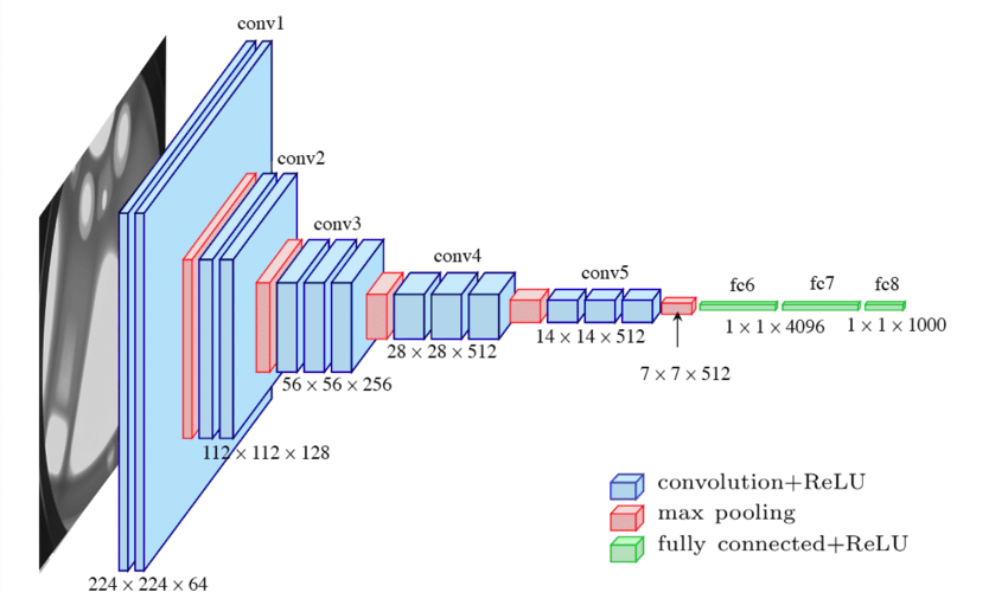
\includegraphics[scale=0.38]{VGGNet1}
\end{figure}

\begin{figure}[htbp]
	\centering
	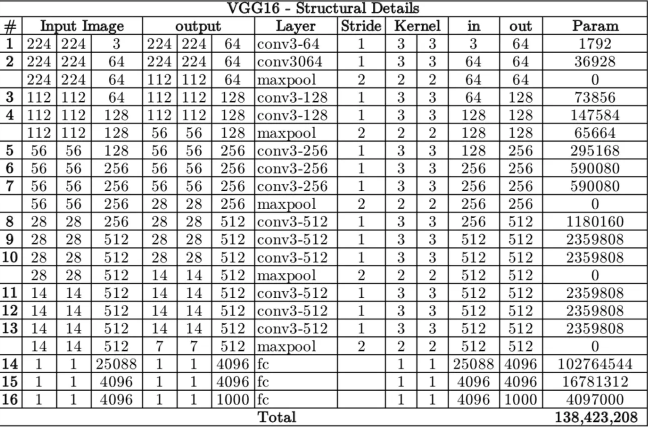
\includegraphics[scale=0.4]{VGGNet2}
\end{figure}

(1)INPUT层:默认输入数据必须是维度为$224\times224\times3$的图像,即输入图像的高度和宽度均为224,色彩通道为R,G,B三个通道。

(2)Conv1层:第一个卷积层,使用的卷积核滑动窗口为$3\times3\times3$,步长为1,Padding为1,可得最后输出的特征图的高度核宽度均为224,这个卷积层输出深度为64的特征图,故需要进行64次同样的卷积操作,最后得到输出的特征图的维度为$224\times224\times64$

(3)MaxPool1层:第一个最大池化层。滑动窗口为$2\times2\times64$,步长为2,,可得最后输出的特征图的高度和宽度均为112,最后得到输出的特征图的维度为$112\times112\times64$

(4)Conv2层:第二个卷积层,使用的卷积核滑动窗口为$3\times3\times64$,步长为1,Padding为1,可得最后输出的特征图的高度核宽度均为112,这个卷积层输出深度为128的特征图,故需要进行128次同样的卷积操作,最后得到输出的特征图的维度为$112\times112\times128$

(5)MaxPool2层:第二个最大池化层。滑动窗口为$2\times2\times128$,步长为2,,可得最后输出的特征图的高度和宽度均为56,最后得到输出的特征图的维度为$56\times56\times128$

(6)Conv3层:第三个卷积层,使用的卷积核滑动窗口为$3\times3\times128$,步长为1,Padding为1,可得最后输出的特征图的高度核宽度均为56,这个卷积层输出深度为256的特征图,故需要进行256次同样的卷积操作,最后得到输出的特征图的维度为$56\times56\times256$

(7)MaxPool3层:第三个最大池化层。滑动窗口为$2\times2\times256$,步长为2,,可得最后输出的特征图的高度和宽度均为28,最后得到输出的特征图的维度为$28\times28\times256$

(8)Conv4层:第四个卷积层,使用的卷积核滑动窗口为$3\times3\times256$,步长为1,Padding为1,可得最后输出的特征图的高度核宽度均为28,这个卷积层输出深度为512的特征图,故需要进行512次同样的卷积操作,最后得到输出的特征图的维度为$28\times28\times512$

(9)MaxPool4层:第四个最大池化层。滑动窗口为$2\times2\times512$,步长为2,,可得最后输出的特征图的高度和宽度均为14,最后得到输出的特征图的维度为$14\times14\times512$

(10)Conv5层:第五个卷积层,使用的卷积核滑动窗口为$3\times3\times512$,步长为1,Padding为1,可得最后输出的特征图的高度核宽度均为14,这个卷积层输出深度为512的特征图,故需要进行512次同样的卷积操作,最后得到输出的特征图的维度为$14\times14\times512$

(11)MaxPool5层:第五个最大池化层。滑动窗口为$2\times2\times256$,步长为2,,可得最后输出的特征图的高度和宽度均为7,最后得到输出的特征图的维度为$7\times7\times512$

(12)FC6层:第一个全连接层。输入特征图的维度为$7\times7\times512$,对输入特征图进行扁平化处理得到$1\times25088$的数据,在经过一个维度为$25088\times4096$的矩阵完成输入数据核输出数据的全连接,最后得到输出数据的维度为$1\times4096$

(12)FC7层:第二个全连接层。输入特征图的维度为$1\times4096$,在经过一个维度为$4096\times4096$的矩阵完成输入数据核输出数据的全连接,最后得到输出数据的维度为$1\times4096$

(13)FC8层:第三个全连接层。输入特征图的维度为$1\times4096$,在经过一个维度为$4096\times1000$的矩阵完成输入数据核输出数据的全连接,最后得到输出数据的维度为$1\times1000$

(14)OUTPUT层:要求最后得到输入图像对应的1000个类别的可能性值。只要将全连接层最后的维度为$1\times100$的数据传递到Softmax激活函数中,就能得到模型预测的输入图像对应1000个类别的可能性值。

\begin{Python}{VGGNet}
	import torch
	import torchvision
	from torchvision import datasets, models, transforms
	import os
	from torch.autograd import Variable
	import matplotlib.pyplot as plt
	import time
	
	data_dir = "Cat_Dog_data"
	data_transform = {x:transforms.Compose([transforms.Resize([224,224]),
		transforms.ToTensor(),
		transforms.Normalize(mean=[0.5,0.5,0.5], std=[0.5,0.5,0.5])])
		for x in ["train", "test"]}
	image_datasets = {x:datasets.ImageFolder(root=os.path.join(data_dir,x),transform=data_transform[x])
		for x in ["train", "test"]}
	dataloader = {x:torch.utils.data.DataLoader(dataset=image_datasets[x],batch_size=16,shuffle=True)
		for x in ["train", "test"]}
	
	X_example, y_example = next(iter(dataloader["train"]))
	example_classes = image_datasets["train"].classes
	index_classes = image_datasets["train"].class_to_idx
	
	model = models.vgg16(pretrained=True)
	
	Use_gpu = torch.cuda.is_available()
	
	for parma in model.parameters():
	parma.requires_grad = False
	
	model.classifier = torch.nn.Sequential(torch.nn.Linear(25088, 4096),torch.nn.ReLU(),torch.nn.Dropout(p=0.5),
	torch.nn.Linear(4096, 4096),torch.nn.ReLU(),torch.nn.Dropout(p=0.5),
	torch.nn.Linear(4096, 2))
	
	if Use_gpu:
	model = model.cuda()
	
	cost = torch.nn.CrossEntropyLoss()
	optimizer = torch.optim.Adam(model.classifier.parameters())
	
	loss_f =torch.nn.CrossEntropyLoss()
	optimizer = torch.optim.Adam(model.classifier.parameters(),lr=0.00001)
	
	epoch_n = 5
	time_open = time.time()
	
	for epoch in range(epoch_n):
	print("Epoch {}/{}".format(epoch, epoch_n-1))
	print("-"*10)
	
	for phase in ["train", "test"]:
	if phase == "train":
	print("Training...")
	model.train(True)
	else:
	print("Testing...")
	model.train(False)
	
	running_loss = 0.0
	running_corrects = 0
	
	for batch, data in enumerate(dataloader[phase], 1):
	x,y=data
	if Use_gpu:
	x,y = Variable(x.cuda()), Variable(y.cuda())
	else:
	x,y = Variable(x),Variable(y)
	y_pred = model(x)
	_,pred = torch.max(y_pred.data, 1)
	optimizer.zero_grad()
	loss = loss_f(y_pred, y)
	if phase == "train":
	loss.backward()
	optimizer.step()
	
	running_loss += loss
	running_corrects += torch.sum(pred == y.data)
	
	if batch%500 == 0 and phase == "train":
	print("Batch {},Train Loss:{:.4f}, Train ACC:{:.4f}".format(batch, running_loss/batch,
	100*running_corrects/(16*batch)))
	
	epoch_loss = running_loss*16/len(image_datasets[phase])
	epoch_acc = 100*running_corrects/len(image_datasets[phase])
	
	print("{} Loss:{:.4f} Acc:{:.4f}%".format(phase, epoch_loss, epoch_acc))
	
	time_end = time.time() - time_open
	print(time_end)
	
	#Output:
	#		Epoch 4/4
	#		----------
	#		Training...
	#		Batch 500,Train Loss:0.0019, Train ACC:99.9625
	#		Batch 1000,Train Loss:0.0025, Train ACC:99.9125
	#		train Loss:0.0037 Acc:99.8978%
	#		Testing...
	#		test Loss:0.0691 Acc:97.8400%
	#		793.4779858589172
	
\end{Python}
\subsubsection{GoogleNet}

\subsubsection{ResNet}
VGGNet尝试探寻深度学习网络究竟可以加深多少以持续地提高分类准确率,但在19层后发现分类准确率下降,后来更多地研究者发现深度神经网络达到一定深度之后再一味地增加层数并不能进一步地使分类性能提高,反而会出现网络性能退化。

ResNet地每一个残差模块都由一系列层和一个捷径连接组成,之歌捷径将该模块地输入特征图和输出特征图连接到一起,并在对应元素地位置上执行加法运算,注意残差模块需要让输入输出特征地形状一致。
\begin{Python}{ResNet}
	import torch
	import torchvision
	from torchvision import datasets, models, transforms
	import os
	from torch.autograd import Variable
	import matplotlib.pyplot as plt
	import time
	
	path = "Cat_Dog_data"
	transform = transforms.Compose([transforms.CenterCrop(224),
	transforms.ToTensor(),
	transforms.Normalize(mean=[0.5,0.5,0.5], std=[0.5,0.5,0.5])])
	data_dir = "Cat_Dog_data"
	data_transform = {x:transforms.Compose([transforms.Resize([224,224]),
		transforms.ToTensor(),
		transforms.Normalize(mean=[0.5,0.5,0.5], std=[0.5,0.5,0.5])])
		for x in ["train", "test"]}
	image_datasets = {x:datasets.ImageFolder(root=os.path.join(data_dir,x),transform=data_transform[x])
		for x in ["train", "test"]}
	dataloader = {x:torch.utils.data.DataLoader(dataset=image_datasets[x],batch_size=16,shuffle=True)
		for x in ["train", "test"]}
	
	X_example, y_example = next(iter(dataloader["train"]))
	example_classes = image_datasets["train"].classes
	index_classes = image_datasets["train"].class_to_idx
	
	model = models.resnet50(pretrained=True)
	
	Use_gpu = torch.cuda.is_available()
	
	for parma in model.parameters():
	parma.requires_grad = False
	
	model.fc = torch.nn.Linear(2048, 2)
	
	if Use_gpu:
	model = model.cuda()
	
	cost = torch.nn.CrossEntropyLoss()
	optimizer = torch.optim.Adam(model.fc.parameters())
	
	loss_f =torch.nn.CrossEntropyLoss()
	optimizer = torch.optim.Adam(model.fc.parameters(),lr=0.00001)
	
	epoch_n = 5
	time_open = time.time()
	
	for epoch in range(epoch_n):
	print("Epoch {}/{}".format(epoch, epoch_n-1))
	print("-"*10)
	
	for phase in ["train", "test"]:
	if phase == "train":
	print("Training...")
	model.train(True)
	else:
	print("Testing...")
	model.train(False)
	
	running_loss = 0.0
	running_corrects = 0
	
	for batch, data in enumerate(dataloader[phase], 1):
	x,y=data
	if Use_gpu:
	x,y = Variable(x.cuda()), Variable(y.cuda())
	else:
	x,y = Variable(x),Variable(y)
	y_pred = model(x)
	_,pred = torch.max(y_pred.data, 1)
	optimizer.zero_grad()
	loss = loss_f(y_pred, y)
	if phase == "train":
	loss.requires_grad_(True)
	loss.backward()
	optimizer.step()
	
	running_loss += loss
	running_corrects += torch.sum(pred == y.data)
	
	if batch%500 == 0 and phase == "train":
	print("Batch {},Train Loss:{:.4f}, Train ACC:{:.4f}".format(batch, running_loss/batch,
	100*running_corrects/(16*batch)))
	
	epoch_loss = running_loss*16/len(image_datasets[phase])
	epoch_acc = 100*running_corrects/len(image_datasets[phase])
	
	print("{} Loss:{:.4f} Acc:{:.4f}%".format(phase, epoch_loss, epoch_acc))
	
	time_end = time.time() - time_open
	print(time_end)
	
	#Output:
	#		Epoch 4/4
	#		----------
	#		Training...
	#		Batch 500,Train Loss:0.1348, Train ACC:96.2375
	#		Batch 1000,Train Loss:0.1323, Train ACC:96.0813
	#		train Loss:0.1315 Acc:96.1156%
	#		Testing...
	#		test Loss:0.0991 Acc:97.2400%
	#		1089.5891721248627
	
\end{Python}
\subsubsection{DenseNet}
\subsubsection{MobileNet}
\subsubsection{ShuffleNet}
\subsection{卷积神经网络案例}
\begin{Python}{CNN案例}
	import torch
	import torch.nn as nn
	from torch.autograd import Variable
	import torch.utils.data as Data
	import torchvision
	import matplotlib.pyplot as plt
	
	EPOCH = 3
	BATCH_SIZE = 50
	LR = 0.001
	DOWNLOAD_MNIST = True
	
	train_data = torchvision.datasets.MNIST(
	root='./mnist/',
	train=True,
	transform=torchvision.transforms.ToTensor(),
	download=DOWNLOAD_MNIST,
	)
	
	#print(train_data.data.size())       #Output:torch.Size([60000, 28, 28])
	#print(train_data.targets.size())    #Output:torch.Size([60000])
	for i in range(1,4):
	plt.imshow(train_data.data[i].numpy(), cmap='gray')
	plt.title('%i' % train_data.targets[i])
	#     plt.show()
	
	#加载数据集
	train_loader = Data.DataLoader(dataset=train_data,batch_size=BATCH_SIZE,shuffle=True)
	
	
	#获取测试集dataset
	test_data = torchvision.datasets.MNIST(root='./mnist/', train=False)
	#加载测试集
	test_x = Variable(torch.unsqueeze(test_data.data, dim=1)).type(torch.FloatTensor)
	test_y = test_data.targets
	
	class CNN(nn.Module):
	def __init__(self):
	super(CNN, self).__init__()
	self.conv1 = nn.Sequential(
	nn.Conv2d(in_channels=1, out_channels=16, kernel_size=5,stride=1, padding=2),
	nn.ReLU(),
	nn.MaxPool2d(kernel_size=2) # (16,14,14)
	)
	self.conv2 = nn.Sequential( # (16,14,14)
	nn.Conv2d(16, 32, 5, 1, 2), # (32,14,14)
	nn.ReLU(),
	nn.MaxPool2d(2) # (32,7,7)
	)
	self.out = nn.Linear(32*7*7, 10)
	def forward(self, x):
	x = self.conv1(x)
	x = self.conv2(x)
	x = x.view(x.size(0), -1) # 将(batch,32,7,7)展平为(batch,32*7*7)
	output = self.out(x)
	return output
	
	cnn = CNN()
	#print(cnn)
	params = list(cnn.parameters())
	# print(len(params))
	# print(params[0].size())
	optimizer = torch.optim.Adam(cnn.parameters(), lr=LR)
	loss_function = nn.CrossEntropyLoss()
	
	for epoch in range(EPOCH):
	for step, (x, y) in enumerate(train_loader):
	b_x = Variable(x)
	b_y = Variable(y)
	output = cnn(b_x)
	loss = loss_function(output, b_y)
	optimizer.zero_grad()
	loss.backward()
	optimizer.step()
	if step % 100 == 0:
	test_output = cnn(test_x)
	pred_y = torch.max(test_output, 1)[1].data.squeeze()
	accuracy = sum(pred_y == test_y) / test_y.size(0)
	print('Epoch:', epoch, '|Step:', step,
	'|train loss:%.4f'%loss, '|test accuracy:%.4f'%accuracy)
	
	test_output =cnn(test_x[:20])
	pred_y = torch.max(test_output, 1)[1].data.numpy().squeeze()
	print(pred_y, 'prediction number')
	print(test_y[:20].numpy(), 'real number')
	
	#Output:
	#       ...
	#		Epoch: 2 |Step: 900 |train loss:0.0623 |test accuracy:0.9855
	#		Epoch: 2 |Step: 1000 |train loss:0.1080 |test accuracy:0.9845
	#		Epoch: 2 |Step: 1100 |train loss:0.1281 |test accuracy:0.9854
	#		[7 2 1 0 4 1 4 9 5 9 0 6 9 0 1 5 9 7 3 4] prediction number
	#		[7 2 1 0 4 1 4 9 5 9 0 6 9 0 1 5 9 7 3 4] real number
	
\end{Python}
\subsection{深度残差模型ResNet案例}
\begin{Python}{ResNet例子}
	import torch
	import torch.nn as nn
	import numpy as np
	import matplotlib.pyplot as plt
	import torchvision.datasets as dsets
	import torchvision.transforms as transforms
	from torch.utils.data import DataLoader
	
	torch.cuda.set_device("cuda:0")
	torch.cuda.current_device()
	
	trans = transforms.Compose([
	transforms.Resize(40),
	transforms.RandomHorizontalFlip(),
	transforms.RandomCrop(32),
	transforms.ToTensor(),
	])
	
	
	train_dataset = dsets.CIFAR10(root='../dataset', train=True, transform=trans, download=True)
	test_dataset = dsets.CIFAR10(root='../dataset', train=False, transform=trans, download=True)
	
	batch_size = 100
	train_loader = DataLoader(dataset=train_dataset, batch_size=batch_size, shuffle=True)
	test_loader = DataLoader(dataset=test_dataset, batch_size=batch_size, shuffle=True)
	
	def conv3x3(in_channels, out_channels, stride=1):
	return nn.Conv2d(in_channels, out_channels, kernel_size=3, stride=stride, padding=1, bias=False)
	
	
	class ResidualBlock(nn.Module):
	def __init__(self, in_channels, out_channels, stride=1, downsample=None):
	super().__init__()
	self.downsample = downsample
	self.conv1 = conv3x3(in_channels, out_channels, stride)
	self.bn1 = nn.BatchNorm2d(out_channels)
	self.relu = nn.ReLU(inplace=True)
	self.conv2 = conv3x3(out_channels, out_channels, stride)
	self.bn2 = nn.BatchNorm2d(out_channels)
	def forward(self, x):
	residual = self.downsample(x) if self.downsample else x
	x = self.relu(self.bn1(self.conv1(x)))
	x = self.bn2(self.conv2(x))
	return self.relu(x + residual)
	
	class ResNet(nn.Module):
	def __init__(self, block, layers, num_classes=10):
	super().__init__()
	self.in_channels = 16
	self.hidden_channels = 16
	self.conv = conv3x3(3, 16)
	self.bn = nn.BatchNorm2d(16)
	self.relu = nn.ReLU(inplace=True)
	self.layer1 = self.make_layer(block, 16, layers[0])
	self.layer2 = self.make_layer(block, 32, layers[1])
	self.layer3 = self.make_layer(block, 64, layers[2], 2)
	self.avg_pool = nn.AvgPool2d(8)
	self.fc = nn.Linear(64, num_classes)
	def forward(self, x):
	x = self.relu(self.bn(self.conv(x)))
	x = self.layer1(x)
	x = self.layer2(x)
	x = self.layer3(x)
	x = self.avg_pool(x)
	x = torch.squeeze(x)
	return self.fc(x)
	def make_layer(self, block, out_channels, blocks_size, stride=1):
	downsample = None
	if stride != 1:
	downsample = nn.Sequential(
	conv3x3(self.hidden_channels, out_channels, stride * 2),
	nn.BatchNorm2d(out_channels),
	)
	elif self.hidden_channels != out_channels:
	downsample = nn.Sequential(
	conv3x3(self.hidden_channels, out_channels, stride),
	nn.BatchNorm2d(out_channels),
	)
	layers = []
	layers.append(block(self.hidden_channels, out_channels, stride, downsample))
	self.hidden_channels = out_channels
	for i in range(1, blocks_size):
	layers.append(block(out_channels, out_channels))
	return nn.Sequential(*layers)
	
	lrate = 0.001
	epochs = 80
	
	model = ResNet(ResidualBlock, [4,4,4]).cuda()
	criterion = nn.CrossEntropyLoss()
	optim = torch.optim.Adam(model.parameters(), lr=lrate)
	
	result = []
	for e in range(epochs):
	for i, (inputs, targets) in enumerate(train_loader):
	inputs = inputs.cuda()
	targets = targets.cuda()
	optim.zero_grad()
	outputs = model(inputs)
	loss = criterion(outputs, targets)
	loss.backward()
	optim.step()
	if i % 50 == 0:
	result.append(float(loss))
	if (i+1) % 100 == 0:
	print('Epoch [%d/%d], Iter [%d/%d] Loss: %.4f' %(e + 1, 80, i+1, 500, loss))
	
	correct = 0
	total = 0
	for i, (inputs, targets) in enumerate(test_loader):
	targets = targets.cuda()
	inputs = inputs.cuda()
	outputs = model(inputs)
	_, preds = torch.max(outputs.data, 1)
	total += len(outputs)
	correct += (preds == targets).sum()
	accuracy = 100 * correct.double() / total
	print('Accuracy of the model on the 10000 test images: %.2f %%' % (accuracy))
	
	#Output:
	#		Epoch [80/80], Iter [200/500] Loss: 0.0882
	#		Epoch [80/80], Iter [300/500] Loss: 0.2076
	#		Epoch [80/80], Iter [400/500] Loss: 0.1064
	#		Epoch [80/80], Iter [500/500] Loss: 0.0601
	#		Accuracy of the model on the 10000 test images: 87.79 %
\end{Python}
\begin{Python}{猫狗识别}

# 导入需要的包
import paddle
import paddle.fluid as fluid
paddle.enable_static()
import numpy as np
from PIL import Image
import sys
from multiprocessing import cpu_count
import matplotlib.pyplot as plt
import os

def unpickle(file):
	import pickle
	with open(file, 'rb') as fo:
	dict = pickle.load(fo, encoding='bytes')
	return dict


print(unpickle("./data/cifar-10-batches-py/data_batch_1").keys())
print(unpickle("./data/cifar-10-batches-py/test_batch").keys())

def test_mapper(sample):
	img, label = sample
	# 将img数组进行进行归一化处理,得到0到1之间的数值
	img = img.flatten().astype('float32') / 255.0
	return img, label

def train_mapper(sample):
	img, label = sample
	# 将img数组进行进行归一化处理,得到0到1之间的数值
	img = img.flatten().astype('float32') / 255.0
	return img, label

def train_r(buffered_size=1024):
	def reader():
		xs = []
		ys = []
		for i in range(1, 6):
			train_dict = unpickle("./data/cifar-10-batches-py/data_batch_%d" % (i,))
			xs.append(train_dict[b'data'])
			ys.append(train_dict[b'labels'])
		
		Xtr = np.concatenate(xs)
		Ytr = np.concatenate(ys)
		
		for (x, y) in zip(Xtr, Ytr):
			yield x, int(y)
		
	return paddle.reader.xmap_readers(train_mapper, reader, cpu_count(), buffered_size)

# 对自定义数据集创建训练集train的reader

def test_r(buffered_size=1024):
	def reader():
		test_dict = unpickle("./data/cifar-10-batches-py/test_batch")
		X = test_dict[b'data']
		Y = test_dict[b'labels']
		for (x, y) in zip(X, Y):
			yield x, int(y)
	return paddle.reader.xmap_readers(test_mapper, reader, cpu_count(), buffered_size)

BATCH_SIZE = 128
# 用于训练的数据提供器
train_reader = train_r()
train_reader = paddle.batch(
							paddle.reader.shuffle(
							reader=train_reader, buf_size=128 * 100),
							batch_size=BATCH_SIZE)
# 用于测试的数据提供器
test_reader = test_r()
test_reader = paddle.batch(
							paddle.reader.shuffle(
							reader=test_reader, buf_size=300),
							batch_size=BATCH_SIZE)



def convolutional_neural_network(img):
	# 第一个卷积-池化层
	conv1 = fluid.layers.conv2d(input=img,  # 输入图像
								num_filters=20,  # 卷积核大小
								filter_size=5,  # 卷积核数量,它与输出的通道相同
								act="relu")  # 激活函数
	pool1 = fluid.layers.pool2d(
								input=conv1,  # 输入
								pool_size=2,  # 池化核大小
								pool_type='max',  # 池化类型
								pool_stride=2)  # 池化步长
	conv_pool_1 = fluid.layers.batch_norm(pool1)
	
	# 第二个卷积-池化层
	conv2 = fluid.layers.conv2d(input=conv_pool_1,
								num_filters=50,
								filter_size=5,
								act="relu")
	pool2 = fluid.layers.pool2d(
								input=conv2,
								pool_size=2,
								pool_type='max',
								pool_stride=2,
								global_pooling=False)
	conv_pool_2 = fluid.layers.batch_norm(pool2)
	# 第三个卷积-池化层
	conv3 = fluid.layers.conv2d(input=conv_pool_2, num_filters=50, 				filter_size=5,act="relu")
	pool3 = fluid.layers.pool2d(
								input=conv3,
								pool_size=2,
								pool_type='max',
								pool_stride=2,
								global_pooling=False)
	# 以softmax为激活函数的全连接输出层,10类数据输出10个数字
	prediction = fluid.layers.fc(input=pool3,
								size=10,
								act='softmax')
	return prediction

# 定义输入数据
data_shape = [3, 32, 32]
images = fluid.layers.data(name='images', shape=data_shape, dtype='float32')
label = fluid.layers.data(name='label', shape=[1], dtype='int64')

# 获取分类器,用cnn进行分类
predict = convolutional_neural_network(images)

# 获取损失函数和准确率
cost = fluid.layers.cross_entropy(input=predict, label=label)  # 交叉熵
avg_cost = fluid.layers.mean(cost)  # 计算cost中所有元素的平均值
acc = fluid.layers.accuracy(input=predict, label=label)  # 使用输入和标签计算准确率

# 获取测试程序
test_program = fluid.default_main_program().clone(for_test=True)
# 定义优化方法
optimizer = fluid.optimizer.Adam(learning_rate=0.001)
optimizer.minimize(avg_cost)
print("完成")


# 定义使用CPU还是GPU,使用CPU时use_cuda = False,使用GPU时use_cuda = True
use_cuda = False
place = fluid.CUDAPlace(0) if use_cuda else fluid.CPUPlace()

exe = fluid.Executor(place)
exe.run(fluid.default_startup_program())

feeder = fluid.DataFeeder(feed_list=[images, label], place=place)

all_train_iter = 0
all_train_iters = []
all_train_costs = []
all_train_accs = []


def draw_train_process(title, iters, costs, accs, label_cost, lable_acc):
	plt.title(title, fontsize=24)
	plt.xlabel("iter", fontsize=20)
	plt.ylabel("cost/acc", fontsize=20)
	plt.plot(iters, costs, color='red', label=label_cost)
	plt.plot(iters, accs, color='green', label=lable_acc)
	plt.legend()
	plt.grid()
	plt.show()


EPOCH_NUM = 4
model_save_dir = "./catdog.inference.model"

for pass_id in range(EPOCH_NUM):
	# 开始训练
	for batch_id, data in enumerate(train_reader()):  # 遍历train_reader的迭代器,并为数据加上索引batch_id
		train_cost, train_acc = exe.run(program=fluid.default_main_program(),  # 运行主程序
		feed=feeder.feed(data),  # 喂入一个batch的数据
		fetch_list=[avg_cost, acc])  # fetch均方误差和准确率
		
		all_train_iter = all_train_iter + BATCH_SIZE
		all_train_iters.append(all_train_iter)
		all_train_costs.append(train_cost[0])
		all_train_accs.append(train_acc[0])
	
		# 每100次batch打印一次训练、进行一次测试
		if batch_id % 100 == 0:
			print('Pass:%d, Batch:%d, Cost:%0.5f, Accuracy:%0.5f' %
			(pass_id, batch_id, train_cost[0], train_acc[0]))
	
	# 开始测试
	test_costs = []  # 测试的损失值
	test_accs = []  # 测试的准确率
	for batch_id, data in enumerate(test_reader()):
		test_cost, test_acc = exe.run(program=test_program,  # 执行训练程序
										feed=feeder.feed(data),  # 喂入数据
										fetch_list=[avg_cost, acc])  # fetch 误差、准确率
		test_costs.append(test_cost[0])  # 记录每个batch的误差
		test_accs.append(test_acc[0])  # 记录每个batch的准确率
	
	# 求测试结果的平均值
	test_cost = (sum(test_costs) / len(test_costs))  # 计算误差平均值(误差和/误差的个数)
	test_acc = (sum(test_accs) / len(test_accs))  # 计算准确率平均值( 准确率的和/准确率的个数)
	print('Test:%d, Cost:%0.5f, ACC:%0.5f' % (pass_id, test_cost, test_acc))

# 保存模型
# 如果保存路径不存在就创建
if not os.path.exists(model_save_dir):
	os.makedirs(model_save_dir)
print('save models to %s' % (model_save_dir))
fluid.io.save_inference_model(model_save_dir,
								['images'],
								[predict],
								exe)
print('训练模型保存完成!')
draw_train_process("training", all_train_iters, all_train_costs, all_train_accs,"trainning cost", "trainning acc")


infer_exe = fluid.Executor(place)
inference_scope = fluid.core.Scope()

def load_image(file):
	# 打开图片
	im = Image.open(file)
	# 将图片调整为跟训练数据一样的大小  32*32,设定ANTIALIAS,即抗锯齿.resize是缩放
	im = im.resize((32, 32), Image.ANTIALIAS)
	# 建立图片矩阵 类型为float32
	im = np.array(im).astype(np.float32)
	# 矩阵转置
	im = im.transpose((2, 0, 1))
	# 将像素值从【0-255】转换为【0-1】
	im = im / 255.0
	# print(im)
	im = np.expand_dims(im, axis=0)
	# 保持和之前输入image维度一致
	print('im_shape的维度:', im.shape)
	return im



with fluid.scope_guard(inference_scope):
	# 从指定目录中加载 推理model(inference model)
	[inference_program,  # 预测用的program
   	 feed_target_names,  # 是一个str列表,它包含需要在推理 Program 中提供数据的变量的名称。
	 fetch_targets] = fluid.io.load_inference_model(model_save_dir, infer_exe)   
	 # fetch_targets:是一个 Variable 列表,从中我们可以得到推断结果。# infer_exe: 运行 inference model的 executor
	
	infer_path = './data/dog.png'
	img = Image.open(infer_path)
	plt.imshow(img)
	plt.show()
	
	img = load_image(infer_path)
	
	results = infer_exe.run(inference_program,  # 运行预测程序
					feed={feed_target_names[0]: img},  # 喂入要预测的img
						fetch_list=fetch_targets)  # 得到推测结果
	print('results', results)
	label_list = [
		"airplane", "automobile", "bird", "cat", "deer", "dog", "frog", "horse",
		"ship", "truck"
	]
	print("infer results: %s" % label_list[np.argmax(results[0])])
	
#OutPut:
#		Pass:3, Batch:300, Cost:0.67910, Accuracy:0.71875
#		Test:3, Cost:0.99540, ACC:0.65872
#		results [array([[0.02856398, 0.01331333, 0.01484357, 0.2511291 , 0.05895644,0.34103772, 0.08130501, 0.1603735 , 0.03779477, 0.01268252]],
#"airplane", "automobile", "bird", "cat", "deer", "dog", "frog", "horse","ship", "truck"
#				dtype=float32)]
#		infer results: dog
\end{Python}
\section{图像风格迁移}
基于卷积神经网络实现图像风格迁移(Style Transfer)的技术也被集成到了相关的应用软件中,吸引了大量的用户参与和体验。

我们首先选取一幅图像作为基准图像即内容图像,然后选取另一幅或多幅图像作为我们希望获得相应风格的图像即风格图像。图像风格迁移的算法就是在保证内容图像的内容完整性的前提下,将风格图像的风格融入内容图像中,使得内容图像的原始风格最后发生转变,最终的输出图像呈现的将是内容图像的内容和风格图像风格之间的理想融合。

\begin{Python}{图像迁移}
	import torch
	import torchvision
	from torchvision import transforms,models
	from PIL import Image
	import matplotlib.pyplot as plt
	from torch.autograd import Variable
	import copy
	
	transforms = transforms.Compose([transforms.Resize([224,224]),
	transforms.ToTensor()])
	
	def loadimg(path = None):
	img = Image.open(path)
	img = transforms(img)
	img = img.unsqueeze(0)
	return img
	
	content_img = loadimg("content/stata.jpg")
	style_img = loadimg("style/wave.jpg")
	assert style_img.size() == content_img.size()
	
	content_img = Variable(content_img).cuda()
	style_img = Variable(style_img).cuda()
	
	class Content_loss(torch.nn.Module):
	def __init__(self, weight, target):
	super(Content_loss, self).__init__()
	self.weight = weight
	self.target = target.detach()*weight
	self.loss_fn = torch.nn.MSELoss()
	
	def forward(self, input):
	self.loss = self.loss_fn(input*self.weight, self.target)
	return input
	
	def bachward(self):
	self.loss.backward(retain_graph = True)
	return self.loss
	
	class Gram_matrix(torch.nn.Module):
	def forward(self, input):
	a,b,c,d = input.size()
	feature = input.view(a*b, c*d)
	gram = torch.mm(feature, feature.t())
	return gram.div(a*b*c*d)
	class Style_loss(torch.nn.Module):
	def __init__(self, weight, target):
	super(Style_loss, self).__init__()
	self.weight = weight
	self.target = target.detach()*weight
	self.loss_fn = torch.nn.MSELoss()
	self.gram = Gram_matrix()
	
	def forward(self, input):
	self.Gram = self.gram(input.clone())
	self.Gram.mul_(self.weight)
	self.loss = self.loss_fn(self.Gram, self.target)
	return input
	
	def backward(self):
	self.loss.backward(retain_graph = True)
	return self.loss
	
	use_gpu = torch.cuda.is_available()
	cnn = models.vgg16(pretrained=True).features
	
	if use_gpu:
	cnn = cnn.cuda()
	
	model = copy.deepcopy(cnn)
	content_layer = ["Conv_3"]
	style_layer = ["Conv_1", "Conv_2", "Conv_3", "Conv_4"]
	content_losses = []
	style_losses = []
	content_weight = 1
	style_weight = 1000
	new_model = torch.nn.Sequential()
	model = copy.deepcopy(cnn)
	gram = Gram_matrix()
	
	if use_gpu:
	new_model = new_model.cuda()
	gram = gram.cuda()
	
	index = 1
	for layer in list(model)[:8]:
	if isinstance(layer, torch.nn.Conv2d):
	name = "Conv_" + str(index)
	new_model.add_module(name, layer)
	if name in content_layer:
	target = new_model(content_img).clone()
	content_loss = Content_loss(content_weight, target)
	new_model.add_module("content_loss_"+str(index), content_loss)
	content_losses.append(content_loss)
	if name in style_layer:
	target = new_model(style_img).clone()
	target = gram(target)
	style_loss = Style_loss(style_weight, target)
	new_model.add_module("style_loss_" + str(index), style_loss)
	style_losses.append(style_loss)
	if isinstance(layer, torch.nn.ReLU):
	name = "Relu_"+str(index)
	new_model.add_module(name, layer)
	index = index+1
	if isinstance(layer, torch.nn.MaxPool2d):
	name = "MaxPool_"+str(index)
	new_model.add_module(name, layer)
	
	input_img = content_img.clone()
	parameter = torch.nn.Parameter(input_img.data)
	optimizer = torch.optim.LBFGS([parameter])
	
	epoch_n = 300
	epoch = [0]
	
	while epoch[0] <= epoch_n:
	def closure():
	optimizer.zero_grad()
	style_score = 0
	content_score = 0
	parameter.data.clamp_(0,1)
	new_model(parameter)
	for sl in style_losses:
	style_score += sl.backward()
	for cl in content_losses:
	content_score += cl.bachward()
	
	epoch[0] += 1
	if epoch[0] % 50 == 0:
	print('Epoch:{} Style Loss: {:4f} Content Loss:{:4f}'.format(epoch[0],style_score.data[0],content_score.data[0]))
	return style_score+content_score
	optimizer.step(closure)
	
	
\end{Python}
	
\end{document}